\Chapter{ARTICLE 1: DORA: DISTRIBUTED ONLINE RISK-AWARE EXPLORER}\label{sec:Theme1}
 

\section{Abstract}
    Exploration of unknown environments is an important challenge in the
    field of robotics. While a single robot can achieve this task alone,
    evidence suggests it could be accomplished more efficiently by
    groups of robots, with advantages in terms of terrain coverage as
    well as robustness to failures. Exploration can be guided through
    belief maps, which provide probabilistic information about which
    part of the terrain is interesting to explore (either based on risk
    management or reward). This process can be centrally coordinated by
    building a collective belief map on a common server. However,
    relying on a central processing station creates a communication
    bottleneck and single point of failure for the system. In this
    paper, we present Distributed Online Risk-Aware (DORA) Explorer, an
    exploration system that leverages decentralized information sharing
    to update a common risk belief map. DORA-Explorer allows a group of
    robots to explore an unknown environment discretized as a 2D grid
    with obstacles, with high coverage while minimizing exposure to
    risk, effectively reducing robot failures.


\section{Introduction}
The exploration of unknown environments is at the core of numerous
robotic applications from search-and-rescue operations
\cite{matos2016multiple} to space
missions~\cite{fong2005interaction}. The problem has been mostly
studied in single robot setups, but the ability to perform exploration
with teams of robots opens the door to even more ambitious
applications, because with proper coordination, the time required to
explore a given environment should decrease proportionally to the
number of robots~\cite{burgard2005coordinated}. Therefore, multi-robot
exploration is an attractive solution to many time-critical
applications such as search-and-rescue operations or planetary
exploration. Moreover, multi-robot teams are usually resilient to some
amount of robot
failures~\cite{ramachandran2019resilience,wehbe2021probabilistic,winfield2006safety}. However,
robot failures are still undesirable as they can affect team
performance and should therefore be avoided, which is the main
motivation for this work, in which we present a risk-aware exploration
algorithm for multi-robot systems: Distributed Online Risk-Aware
(DORA) Explorer.

Multi-robot systems come with their own sets of constraints and
challenges: among those, coordination and communication are the most
relevant to the exploration problem. Without coordination, the robots
will inevitably explore overlapping parts of the environment, leading
to little gains in terms of efficiency compared to single-robot
solutions. While the coordination could be optimally orchestrated from
a central computing station, such a solution would require a perfect
connectivity maintenance with each robot and a high communication
bandwidth since the robots would need to send their observations and
receive their commands. This motivates the need for a decentralized
exploration algorithm relying only on local computation onboard the
robots and communication with their neighbours. To the best of our knowledge, there exists no risk-aware collaborative
exploration algorithm that relies solely on local or shared
information. Therefore, in this paper, we make the following
contribution to the field of multi-robot exploration: \textit{A
  decentralized exploration algorithm leveraging distributed belief
  maps (DBMs) to maximize coverage and decrease robot failure
  probability using risk-awareness.} To
evaluate this system, we test it on the specific problem of
\emph{hazard mapping} in a 2D world discretized as a grid, in which a
multi-robot team simultaneously explores a dangerous environment and
collaborates to avoid hazardous locations as well as obstacles. We validate our approach in a physics-based simulator, ARGoS
\cite{Pinciroli:SI2012}, in which we define a grid-based environment
with multiple radiation sources. We then test it on physical
robots and obtain convincing results. 

\section{Related Work and Background}
Distributed sensing and information sharing is not trivial, especially considering
the challenges of consistency and partial connectivity among the
robotic teams~\cite{amigoni2017multirobot,otte2018emergent}. The virtual stigmergy
presented in \cite{pinciroliTuple2016} and implemented in the Buzz
programming language \cite{pinciroliBuzz2016} achieves consensus among
a group of robots using Conflict-free Replicated Data Types (CRDTs),
represented as key-value pairs shared and replicated among the swarm members. This sort of shared data structure is
particularly relevant for belief maps, since it is easy to assign a
unique key to each cell based on its location.  In the virtual
stigmergy, data is shared on writing and reading the CRDT, with the
additional updates on read improving the robustness to temporary
disconnections and message drops. This solution differs from
distributed hash tables, which require a complete view of the system
at every point in time. Essentially, information updates are propagated throughout the swarm using the stigmergy whenever it is possible. In this sense, it offers high availability while settling for eventual data consistency. Other distributed data storage approaches such
as SwarmMesh \cite{majcherczykSwarmmesh2020} store data in different
locations based on a fitness function instead of replicating them on
all robots. This allows the storage of more data with less
communication, but robots are less likely to have access to the latest
values.

Belief maps are a simple yet powerful tool for robotic exploration
because they can represent an environment with a 2D cell grid. They
are a generalization of occupancy maps: instead of storing only one
bit per cell to indicate the presence of an obstacle/danger, they
store obstacle/danger likelihoods and offer significant improvements
for exploration \cite{stachnissMappingExplorationMobile2003}. In the
field of multi-robot exploration, early techniques leveraging belief
maps date back as far as twenty years
\cite{kobayashiSharingExploringInformation2002,kobayashiDeterminationExplorationTarget2003},
but they rely on a fixed grid size and are tested only with two
robots. More recent works also leverage belief maps for multi-robot
exploration. For example,
in~\cite{indelmanCooperativeMultirobotBelief2018}, the robots consider
both the current beliefs and the expected beliefs from future
observations to coordinate their exploration. Grid maps and belief
maps are also widely used to train deep reinforcement learning
exploration policies
\cite{hanGridWiseControlMultiAgent,panovGridPathPlanning2018}, but they often rely on a trial and error process which may select actions leading to failures \cite{garciaSafeExplorationState2012,andersenSafeReinforcementlearningIndustrial2020}.

To provide more insight into our claim that there are no risk-aware collaborative exploration strategies in  the literature, it should be noted that risk-awareness has indeed been used in some swarm systems to improve robustness. For example, several path planners based on Markov Decision Processes \cite{undurti2010online,thiebaux2016rao,xiao2020robot} take into account risk and have useful definitions of it. Another interesting idea for risk awareness is proposed in \cite{ono2008efficient,vitus2011feedback}, where a "risk budget" is allocated to their agents, allowing them to optimize a balance between risk and reward to guide robots. However, these systems assume a knowledge of the global state of the environment, which is unavailable when exploring unknown environments. Furthermore, most are only applied to single-robot systems. In SPIDER \cite{hunt2020spider}, multiple agents are tasked with chain formation in dangerous environments. They adapt to varying levels of risk to be resilient to significant failures and member losses. However, their task is significantly different from DORA Explorer's objectives.

Many distributed exploration strategies maximizing the amount of
covered terrain have been proposed. The first approaches to stand out
in this regard are Voronoi-based coverage control
techniques~\cite{luo2019voronoi,santos2019decentralized}. A second
method covers time-varying domains, in which points in the
covered region can become more or less interesting to explore,
therefore prompting a change in the coverage function
\cite{santos2019decentralized,xu2019multi}. Another method to optimize
coverage is Frontier-Based Exploration (FBE)
\cite{yamauchi1998frontier} of which many variations have been
developed, such as those based on Particle Swarm Optimization
\cite{wang2011frontier} or the Wavefront Frontier Detector
\cite{topiwala2018frontier}. However, none of these strategies take
risk into account. Therefore, the
exploration strategy implemented in this paper takes inspiration of
the multi-robot control algorithm presented in
\cite{dames2012decentralized,schwagerMultirobotControlPolicy2017}
which maximizes the information gain during exploration in the
presence of unknown hazards. However, this optimal algorithm has a
very high computational complexity and could benefit from approximations.

% We build on those approaches and address some their shortcomings by
% implementing a risk-aware exploration algorithm leveraging a DBM of
% the environment which is not constrained to a fixed size.


\section{System Model}
DORA-Explorer builds on the previously mentioned approaches and addresses some of their shortcomings, namely by leveraging risk awareness to provide better efficiency when exploring hazardous environments. Reducing the
likelihood of robot failures is of high importance as they lead to poor exploration performance. Indeed, if robots experiencing complete
failures are not replaced, individual failures lead to lower numbers
of robots carrying the exploration task resulting in a decrease of the exploration rate. We model the 2D environment as cells forming a grid
represented as $E \subset \mathbb{Z}^2$. The team of robots is denoted
as the collection of agents $a_i \in A$.

% \begin{figure*}[h]
%     \centering
%     % \begin{subfigure}{0.40\textwidth}
%     %      \centering
%     %      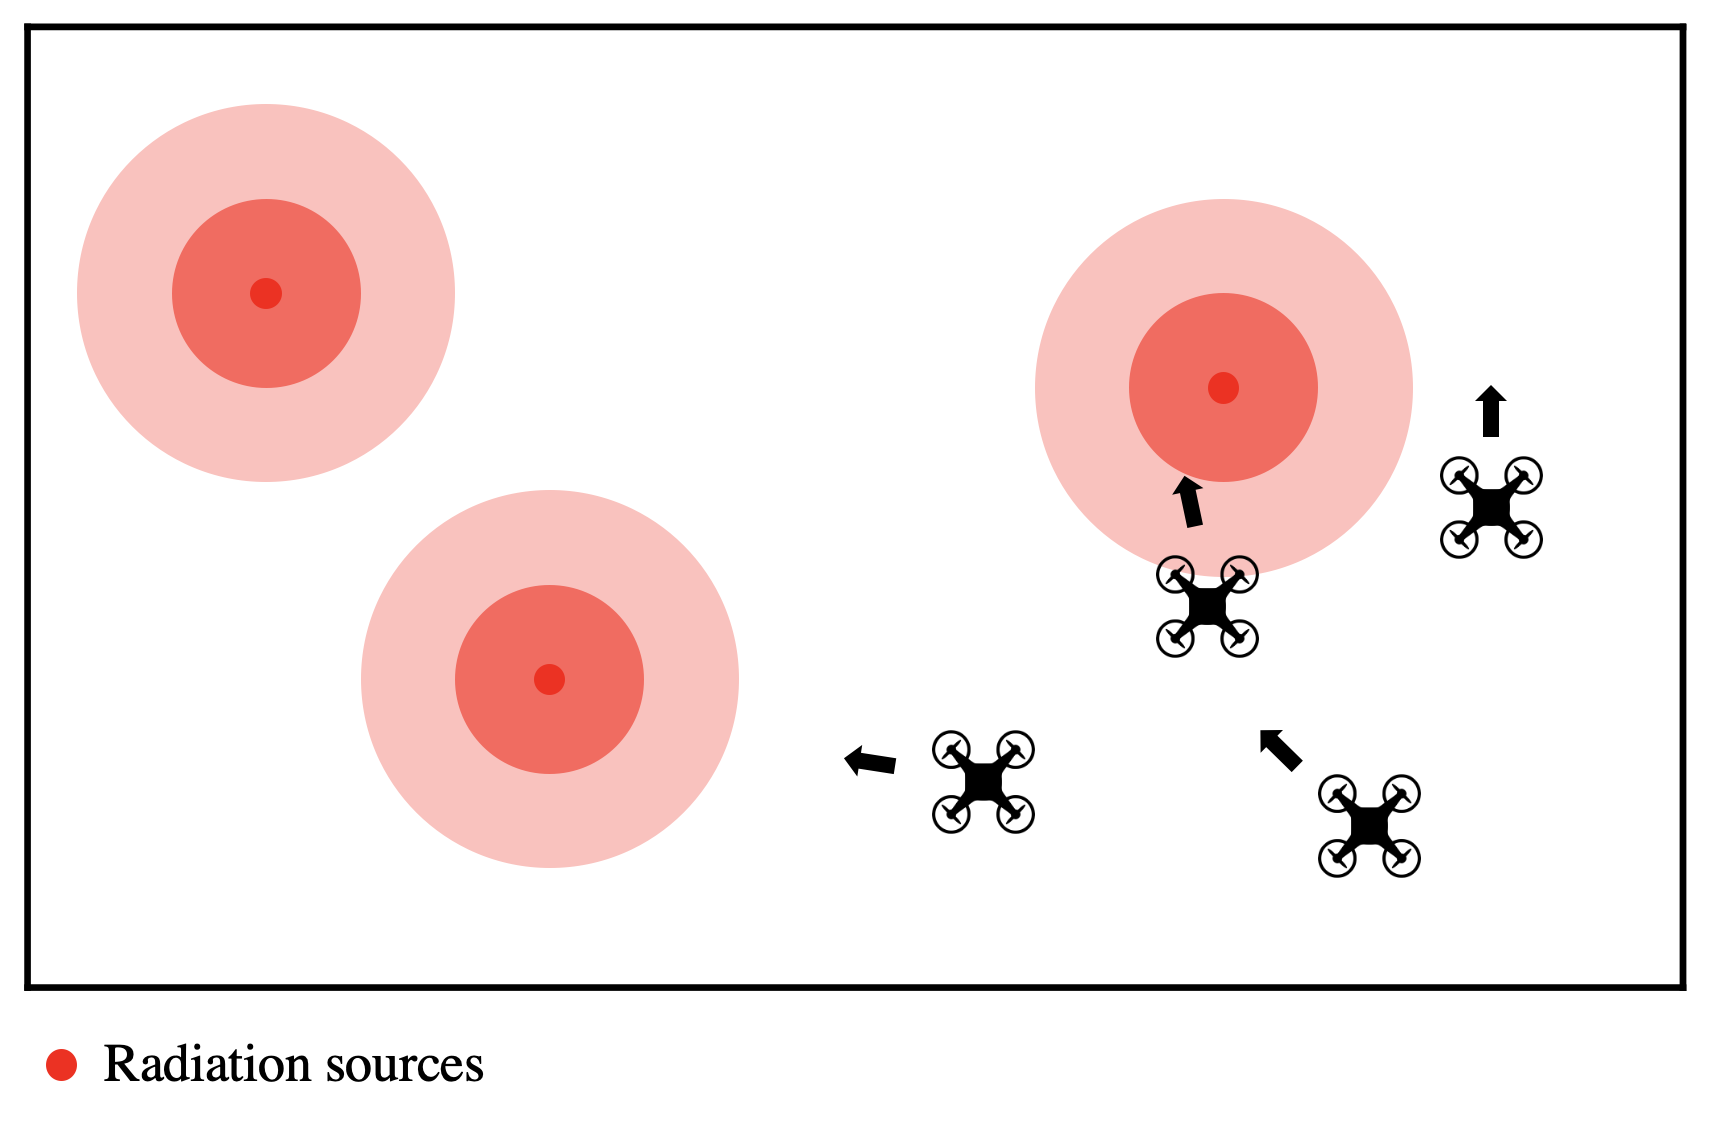
\includegraphics[width=\textwidth]{images/risk_aware_a.png}
%     %      \caption{}
%     %      \label{risk_aware_a}
%     % \end{subfigure}
%     % \hfill
    
    
%     \begin{subfigure}{0.30\textwidth}
%          \centering
%          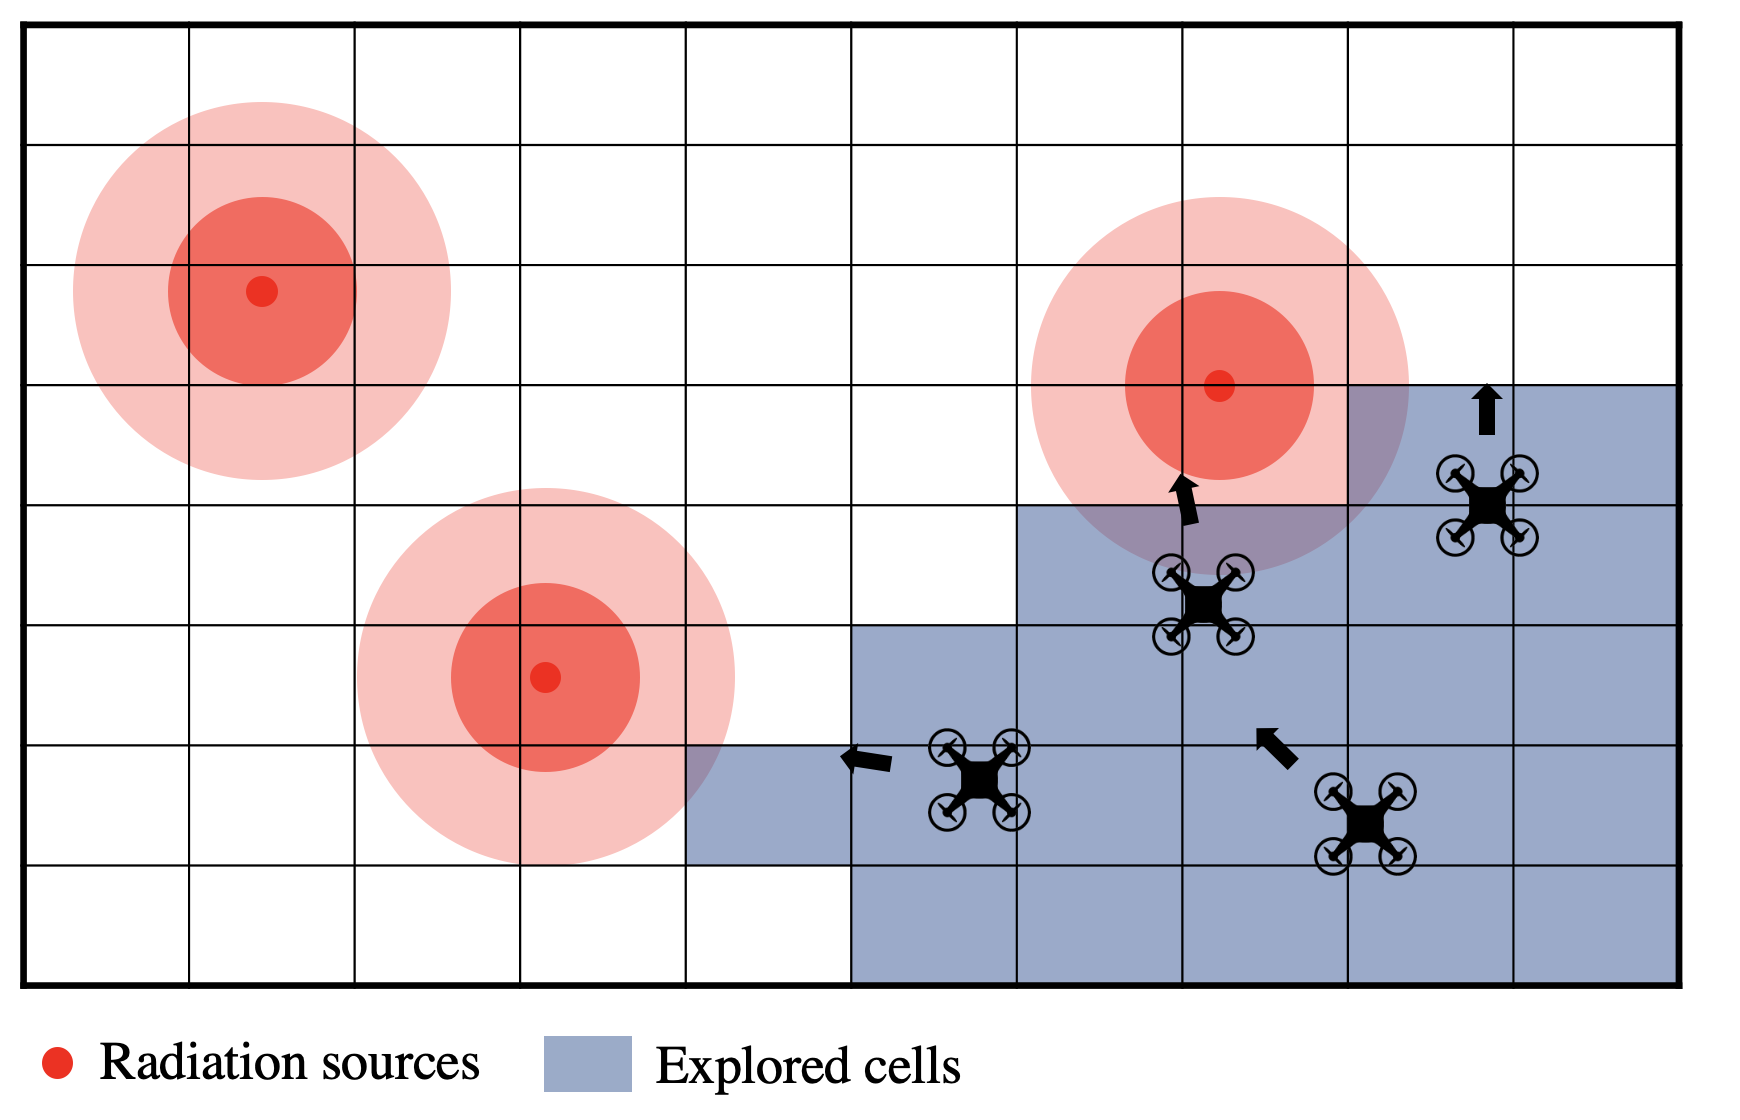
\includegraphics[width=\textwidth]{images/risk_aware_b.png}
%          \caption{}
%          \label{risk_aware_b}
%     \end{subfigure}
%     \hfill
%     \begin{subfigure}{0.30\textwidth}
%          \centering
%          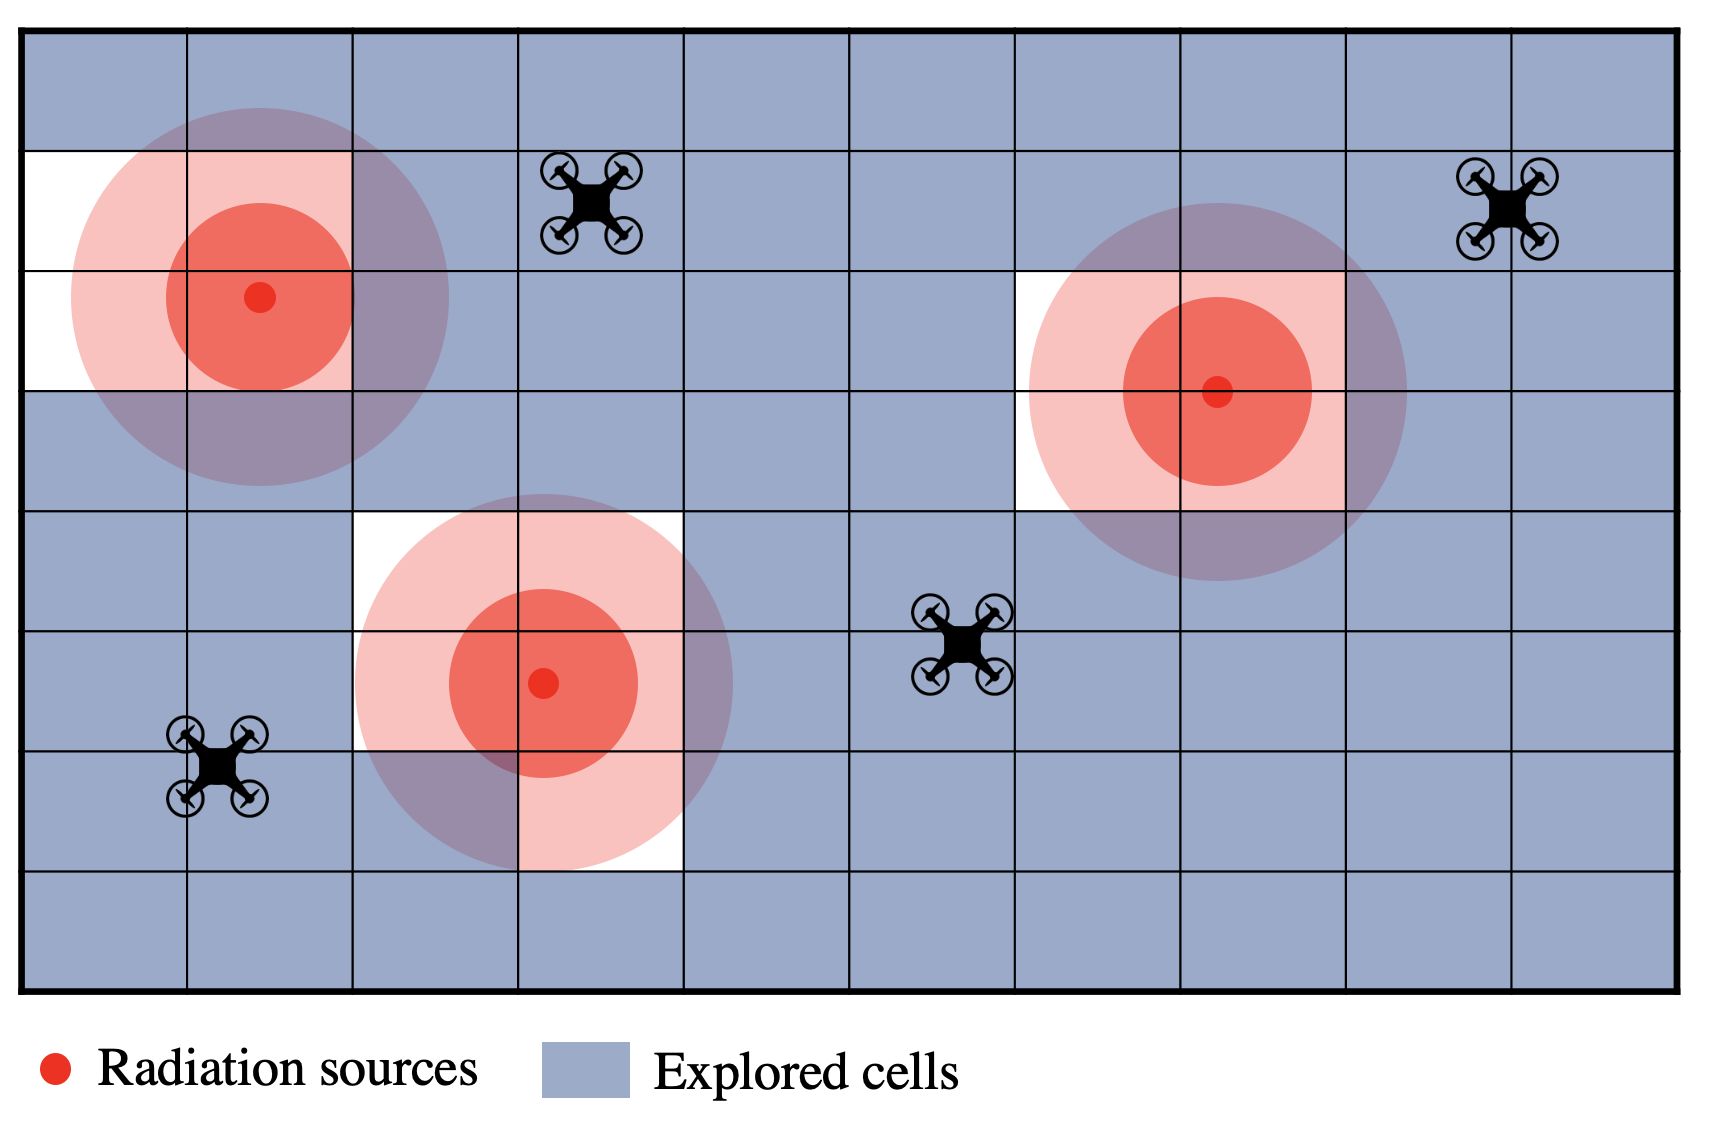
\includegraphics[width=\textwidth]{images/risk_aware_c.png}
%          \caption{}
%          \label{risk_aware_c}
%     \end{subfigure}
%     \hfill
%     \begin{subfigure}{0.30\textwidth}
%          \centering
%          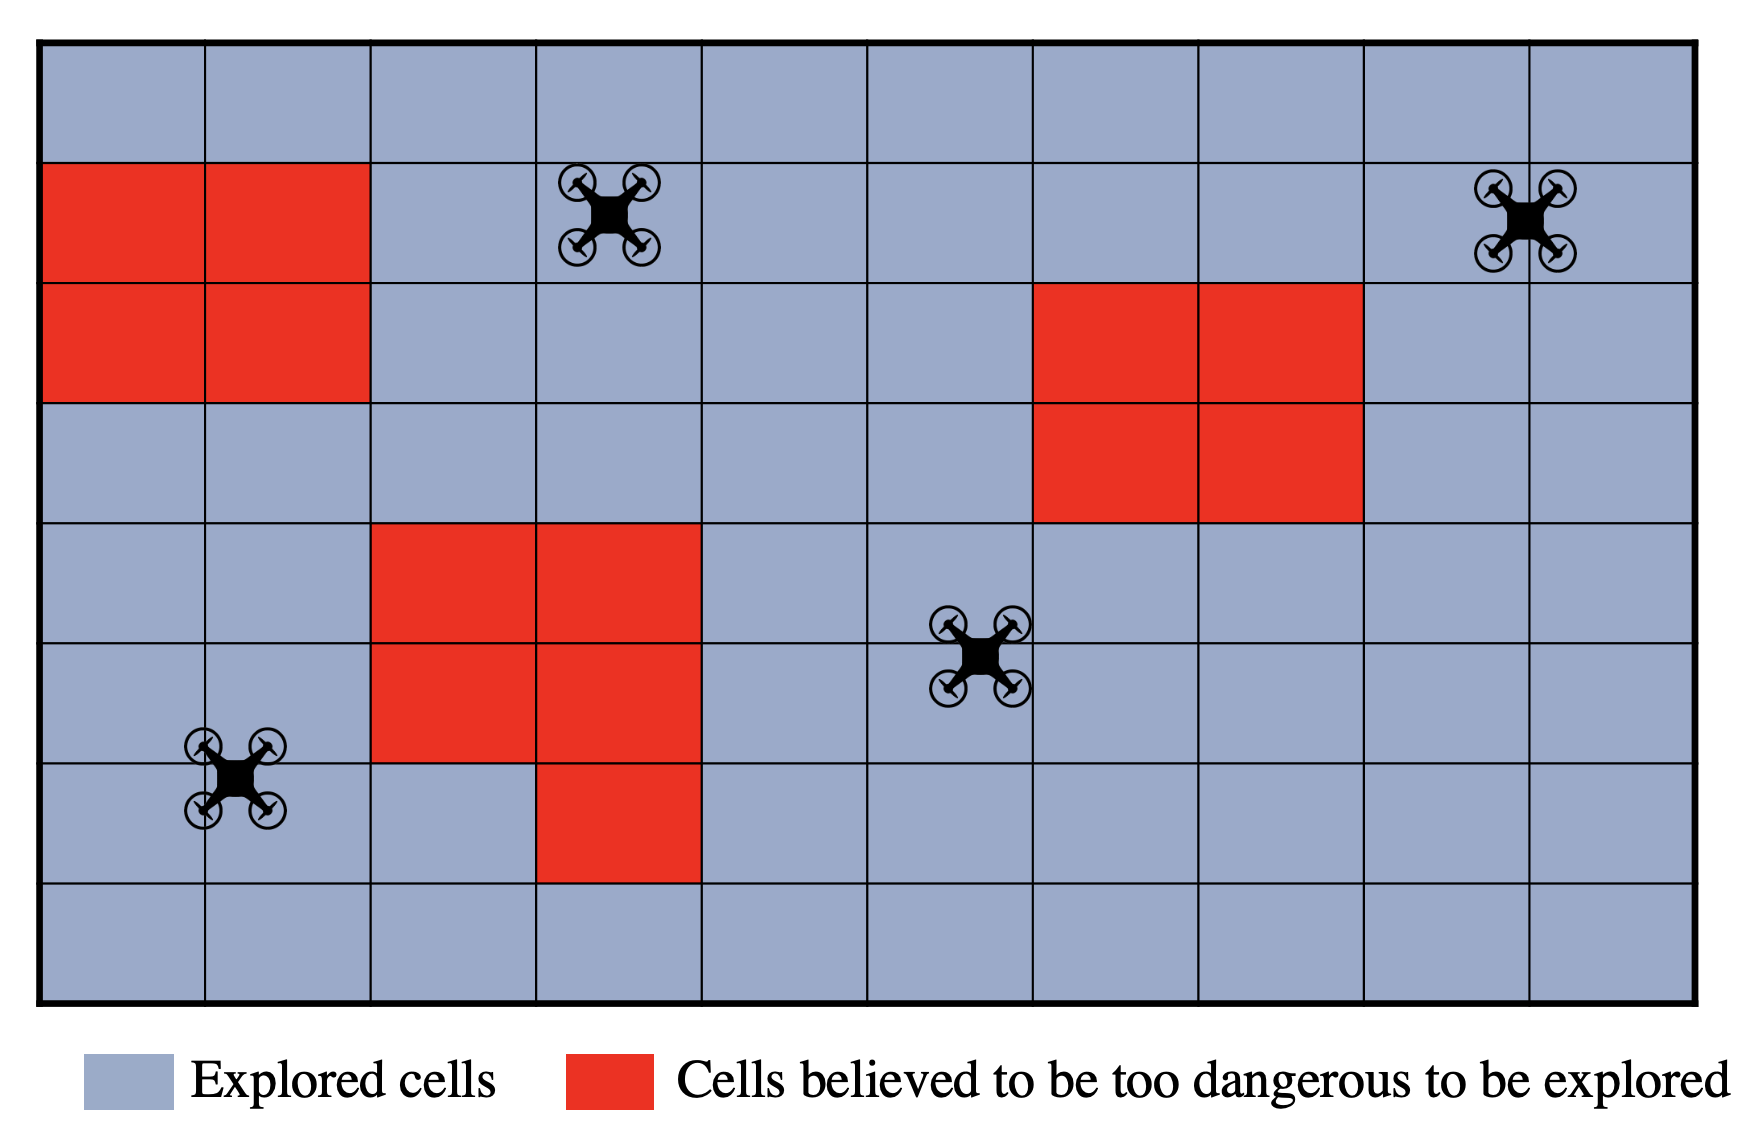
\includegraphics[width=\textwidth]{images/risk_aware_d.png}
%          \caption{}
%          \label{risk_aware_d}
%     \end{subfigure}
%         \caption{Risk aware exploration intuition. Fig. \ref{risk_aware_b}: Robots start exploring a hazardous environment. When a new cell is explored, the sensed radiation is used to update the DBM. Fig. \ref{risk_aware_c}: The cells have been mostly covered by the robots. Fig. \ref{risk_aware_d}: Only cells believed to be too dangerous remain unexplored.}
%     \label{risk_aware}
% \end{figure*}


\subsection{Risk Modelling}
Without loss of generality, we model risk considering point radiation
sources, denoted by the set $S$. The intensity of each radiation
source is given by $I_j\sim\mathcal{U}(0, 1)$. Each source's position
is denoted by $\bm{s}_j \in E$. Given a robot $a_i$'s discrete
position $\bm{x}_i \in E$, the perceived radiation level by that robot coming from radiation source $\bm{s}_j$ is given by:

\begin{equation}
    r_{\bm{s}_j}(\bm{x}_i) = \frac{I_j}{1 + \lambda\rho^2}
    \label{eq:radiation}
\end{equation}

which decays as the distance $\rho$ between $\bm{s}_j$ and $\bm{x}_i$
increases, and $\lambda$ is a decay constant. Measurement noise is
accounted for in the form of a Gaussian background radiation
$b \sim \mathcal{N}(0, 0.05)$. The total radiation perceived by a robot is:

\begin{equation}
    r(\bm{x}_i) = b + \sum_{\bm{s}_j \in S} r_{\bm{s}_j}(\bm{x}_i)
\end{equation}

Robots are only able to sense the radiation level associated with
their current position using an onboard sensor. They do not hold any
knowledge of where the radiations sources are located in the
environment. For the following definitions, it should be noted that
$r_{s_j}: E \rightarrow [0, 1]$.  Let
the event of robot $a_i$ failing be $f_i=1$, the probability of such a
failure due to an individual source of radiation follows a Bernoulli
distribution:
$\mathbb{P}(f_i = 1 | \bm{s}_j) \sim
\mathcal{B}(r_{\bm{s}_j}(\bm{x}_i))$. We assume that the sources of
radiation affect the robots independently, consequently the probability of a
robot failing due to the combined effect of all radiation sources is:

\begin{equation}
    \mathbb{P}(f_i = 1 | S) = 1 - \prod_{\bm{s_j} \in S} (1 - \mathbb{P}(f_i = 1 | \bm{s}_j))
    \label{eq:failure}
\end{equation}

\subsection{Information Modelling}
The objective of exploring an unknown dynamic environment is to gain
information about it. Moreover, this information should be as up to
date as possible. Therefore, it is unlikely that visiting a recently
explored cell will yield any significant gain as the information
should not have changed drastically. Conversely, exploring areas
visited long ago should yield a greater information gain, and
unvisited areas should provide the highest information gain. The last
time of exploration $t_\epsilon$ by robot $a_i$ of a cell at position
$\bm{x}_i$ can be represented by the scalar field
$\epsilon(\bm{x}_i) = t_\epsilon$. Let $u_i=1$ be the event of robot
$a_i$ finding useful information in a cell and
$\Delta t = t-t_\epsilon$ the time elapsed since the cell was last
visited, with $t$ being the current time. Then, the probability of
\textit{not} finding useful information
$\mathbb{P}(u_i=0 | f_i=0, \Delta t)$ can be modelled as an
exponential distribution with the following probability density
function:

\begin{equation}
    f(\Delta t;\omega) = \omega e^{-\omega\Delta t}
    \label{eq:information}
\end{equation}

where $\omega$ is the rate parameter of the distribution. In words,
the longer the cell has not been visited, the higher the chance
something has changed and consequently the lower the chance of not
finding useful information. Intuitively, no information can be acquired by failed robots.

\subsection{Distributed Belief Map}
To implement a DBM, we use the virtual
stigmergy~\cite{pinciroliTuple2016} from the
Buzz~\cite{pinciroliBuzz2016} programming language. Because
$r(\bm{x}_i)$ and $\epsilon(\bm{x}_i)$ are both scalar fields, they
lend themselves particularly well to being stored in a CRDT at a low
cost. At each time step, the robots store their values of
$r(\bm{x}_i)$ and $\epsilon(\bm{x}_i)$ in their respective
stigmergies.  The inputs to both fields are used as keys in the distributed belief map (more precisely, a concatenation of $\bm{x}_{i;x}$ and $\bm{x}_{i;y}$). This
means that the cost of storing the information for a given time step
is very low, especially as the keys consist of a few characters and
the values are floating point numbers. Storing the information into
the DBM via the virtual stigmergy allows robots to share their
observations as it is accessible by every robot in the system. Thus, a
robot visiting a cell for the first time could still have information from
which to compute a good control policy if this cell was previously
visited by another robot. In the event of a collision in the stigmergy
(when robots write to the same key in the same $t$), the robot making the latest observation updates the table. When a robot writes to a key already present
in the stigmergy (from a previous time step), the new data is merged
with an average and the result is propagated. A running average was used to update the belief map because of the noisy readings. 

\subsection{Control Law}
We assume that robots can be controlled through a position-based
control law. The best control policy should attempt to minimize
probability of failure and to maximize information gain. While the
directions achieving these individual objectives might be at odds in
the short term, they are in fact complementary in the long term
because no information can be gained if a robot failed, which means that avoiding danger
implicitly leads to more opportunities of gaining information
\cite{schwagerMultirobotControlPolicy2017}.

\begin{figure}[h]
	\centering
    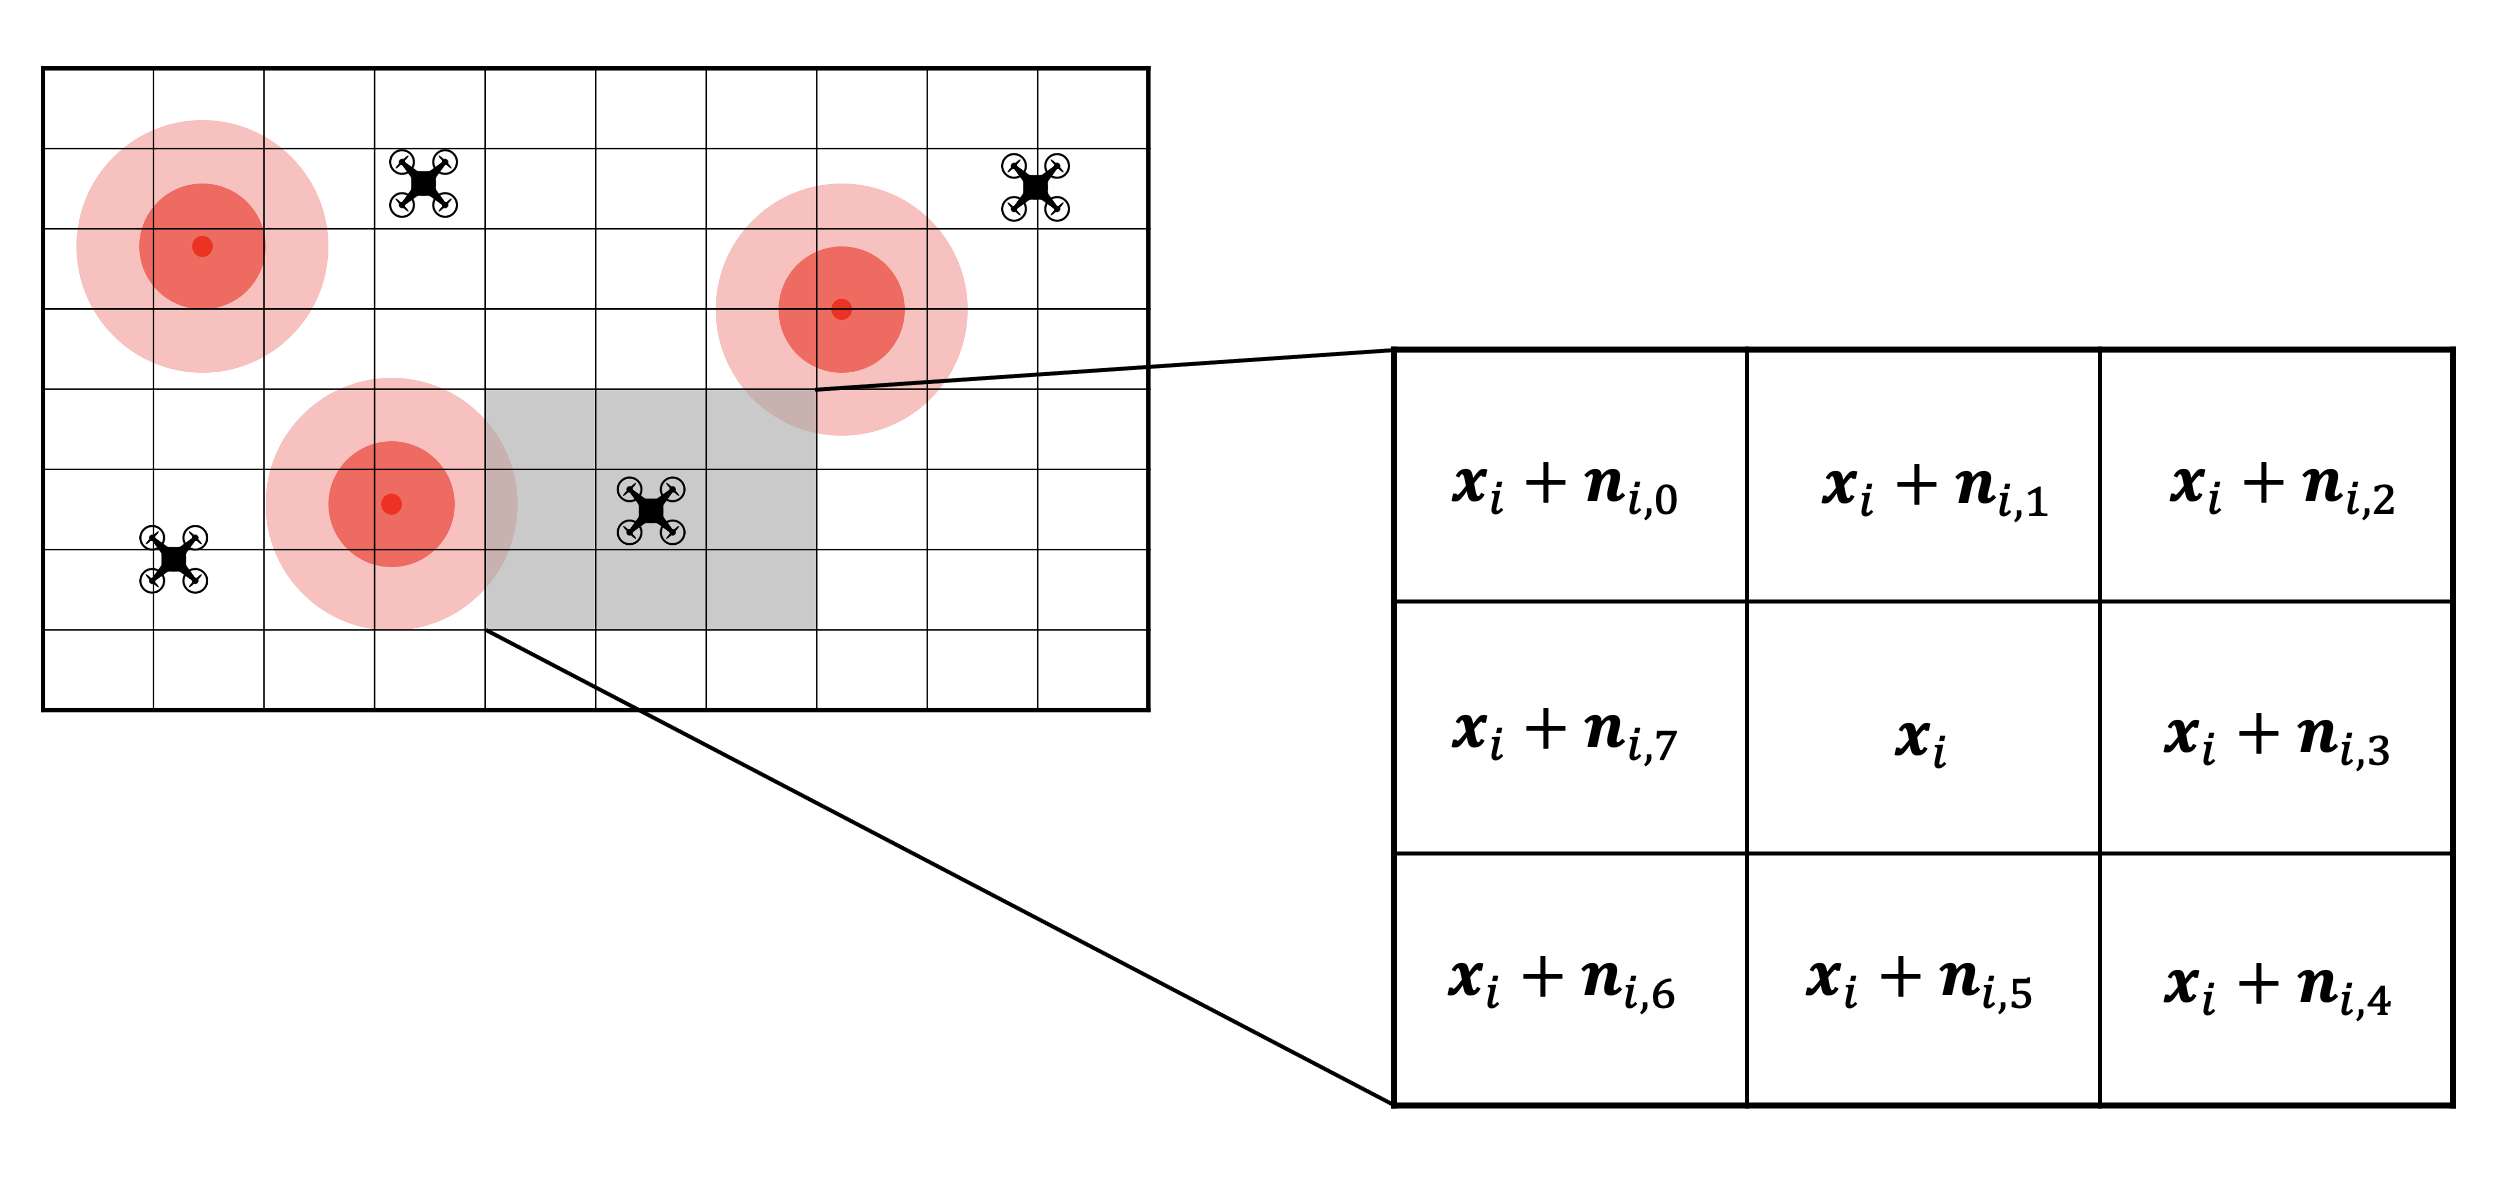
\includegraphics[width=0.95\columnwidth]{images/Moore.png}
    \caption{$\bm{x}_i$'s neighborhood. $\bm{n}_{i,0} = (-1, 1)$ is neighbor 0's offset from $\bm{x}_i$.}
    \label{neighborhood}
\end{figure}

For a robot at a given position $\bm{x}_i$, the directions where the
risk is minimized and the information gain is maximized are
respectively $\bm{\nabla}r(\bm{x}_i)$ and
$\bm{\nabla}\epsilon(\bm{x}_i)$, also denoted as $\bm{\nabla}_{r;i}$
and $\bm{\nabla}_{\epsilon;i}$. Calculating these globally at every
time step is too computationally expensive
\cite{dames2012decentralized,schwagerMultirobotControlPolicy2017}. Instead,
we compute them locally in a Moore neighborhood $\nu$ centered on
$\bm{x}_i$ as shown in Fig. \ref{neighborhood} where each neighboring
cell $\bm{n}_{i,j} \in \nu$ is a vector in $\mathbb{Z}^2$ representing
an offset from $\bm{x}_i$. We then have:

\begin{equation}
    \bm{\nabla}_{r;i} = \sum_{\bm{n}_j \in \nu}\frac{\partial r}{\partial \bm{n}_{i,j}} \bm{\hat{n}}_{i,j} \text{ , with } \frac{\partial r}{\partial \bm{n}_{i,j}} = r(\bm{x}_i) - r(\bm{n}_{i,j})
    \label{eq:gradient_risk}
\end{equation}

\begin{equation}
    \bm{\nabla}_{\epsilon;i} = \sum_{\bm{n}_j \in \nu}\frac{\partial \epsilon}{\partial \bm{n}_{i,j}} \bm{\hat{n}}_{i,j} \text{ , with } \frac{\partial \epsilon}{\partial \bm{n}_{i,j}} = \epsilon(\bm{x}_i) - \epsilon(\bm{n}_{i,j})
    \label{eq:gradient_exploration}
\end{equation}

% \begin{equation}
%     \frac{\partial r}{\partial \bm{n}_{i,j}} = r(\bm{x}_i) - r(\bm{n}_{i,j})
%     \label{eq:neighbor}
% \end{equation}

% \begin{equation}
%     \bm{\nabla}_{r;i} = \sum_{\bm{n}_j \in \nu}\frac{\partial r}{\partial \bm{n}_{i,j}} \bm{\hat{n}}_{i,j}
%     \label{eq:gradient}
% \end{equation}

% \begin{equation}
%     \frac{\partial \epsilon}{\partial \bm{n}_{i,j}} = \epsilon(\bm{x}_i) - \epsilon(\bm{n}_{i,j})
%     \label{eq:neighbor}
% \end{equation}

% \begin{equation}
%     \bm{\nabla}_{\epsilon;i} = \sum_{\bm{n}_j \in \nu}\frac{\partial \epsilon}{\partial \bm{n}_{i,j}} \bm{\hat{n}}_{i,j}
%     \label{eq:gradient}
% \end{equation}

where $\bm{\hat{n}}$ is the unit form of $\bm{n}$. Neighboring cells that have never been visited before are simply ignored when determining the gradients. If none of the neighboring cells have been explored yet, or if the computed direction is null, the robot simply moves forward until it's able to compute a meaningful direction. The movement vector $\bm{m}_i \in \mathbb{R}^2$ for the next time step
gives a good approximation for short term trajectory planning and is given by:

\begin{equation}
    \bm{m}_i = \alpha\bm{\nabla}_{r;i} + \beta\bm{\nabla}_{\epsilon;i} + \gamma\bm{o}_i
    \label{eq:movement}
\end{equation}

where $\alpha, \beta, \gamma$ are respectively the risk avoidance,
exploration and obstacle avoidance control gains. The parameters can
be adjusted arbitrarily; setting them to zero removes the effect
of the corresponding control law. The obstacle avoidance vector was
included to insure robustness and is taken from
\cite{shahriari2018lightweight}. With $\bm{\hat{m}_i}$ being the
normalized vector movement and $k$ a speed constant, the control law
for an agent $a_i$ at time step $t$ is expressed as:

\begin{equation}
    \bm{x}_i^{t+1} = \bm{x}_i^t + k \bm{\hat{m}}_i^t
    \label{eq:control}
\end{equation}

A constant search speed enables a fair comparison with the baselines detailed in section \ref{experimentSetup} as the exploration capabilities of the robots remain the same across the algorithms.

% \subsection{Implementation}
% The DBMs and the control law previously described are combined to create the behavior of an agent. At every
% time step, the information from the DBMs is used to determine the
% agent's next movement. The DBMs are then updated with the new
% information gained. Global exploration efficiency emerges through the
% exchange of information through the stigmergies, but no explicit
% coordination is required otherwise. Unlike FBE algorithms, DORA-Explorer never
% stops exploring the environment even if all cells are covered, as
% information could be gained by visiting "old" cells. If
% $\|\bm{\hat{m}}_i\|$ is too small, the agents move forward to avoid
% stagnation.

% \begin{algorithm}[h]
% \small
% \SetAlgoLined
% \DontPrintSemicolon
%  $\bm{x} \leftarrow random\_coordinates$\;
%  \While{True}{
%   $\nabla_r, \nabla_e \longleftarrow (0, 0), (0, 0)$\;
%   \;
%   \For{$n \in \nu$}{
%     $\nabla_r \leftarrow \nabla_r + (r\_stig[\bm{x}] - r\_stig[\bm{n}]) \cdot normalize(\bm{n})$\;
%     $\nabla_e \leftarrow \nabla_e + (e\_stig[\bm{x}] - e\_stig[\bm{n}]) \cdot normalize(\bm{n})$\;
%   }
%   \;
%   $\bm{m} \leftarrow \alpha \cdot \nabla_r + \beta \cdot \nabla_e + \gamma \cdot compute\_avoidance(sensors)$\;
%   $\bm{x} \leftarrow \bm{x} + k \cdot normalize(\bm{m})$\;
%   $r\_stig[\bm{x}], e\_stig[\bm{x}] \leftarrow get\_radiation(), time()$\;
%  }
%  \caption{DORA-Explorer Execution Loop}
%  \label{alg:dora}
% \end{algorithm}


% \begin{figure*}
%      \centering
%      \begin{subfigure}{0.30\textwidth}
%          \centering
%          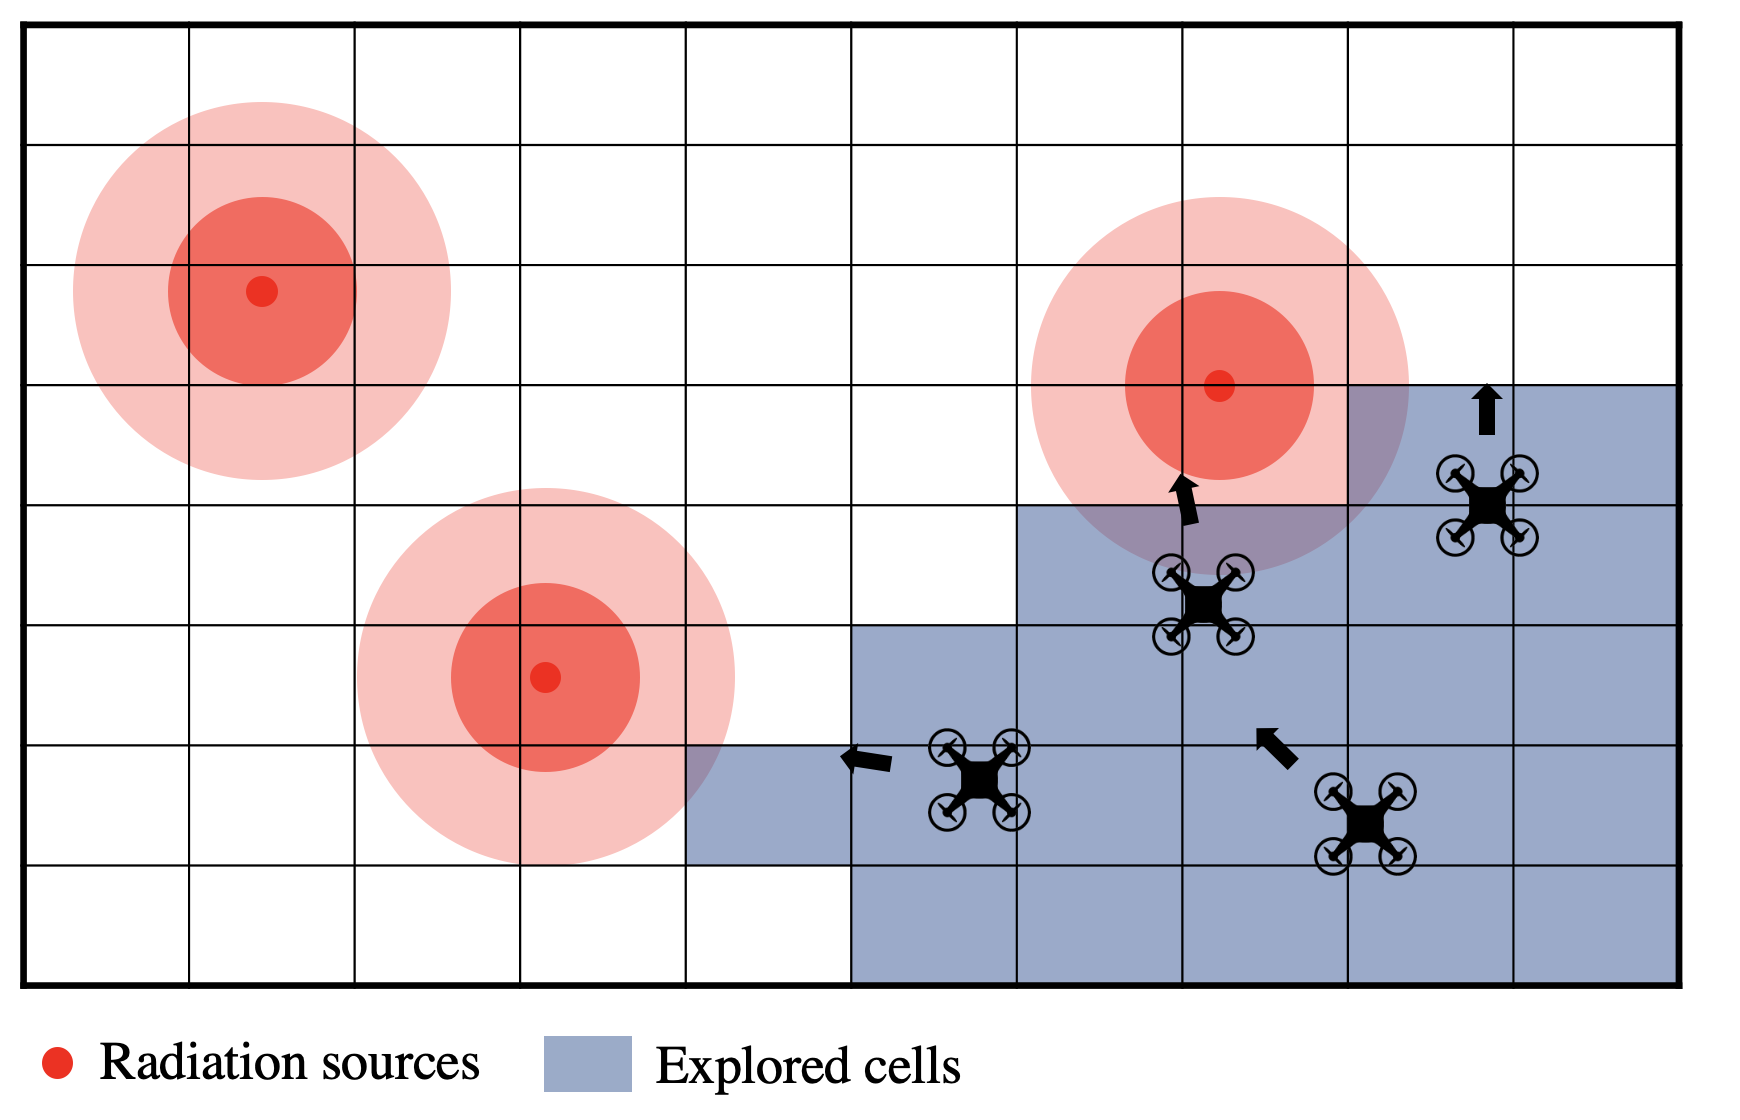
\includegraphics[width=\textwidth]{images/risk_aware_b.png}
%          \caption{}
%          \label{risk_unaware_a}
%      \end{subfigure}
%      \begin{subfigure}{0.30\textwidth}
%          \centering
%          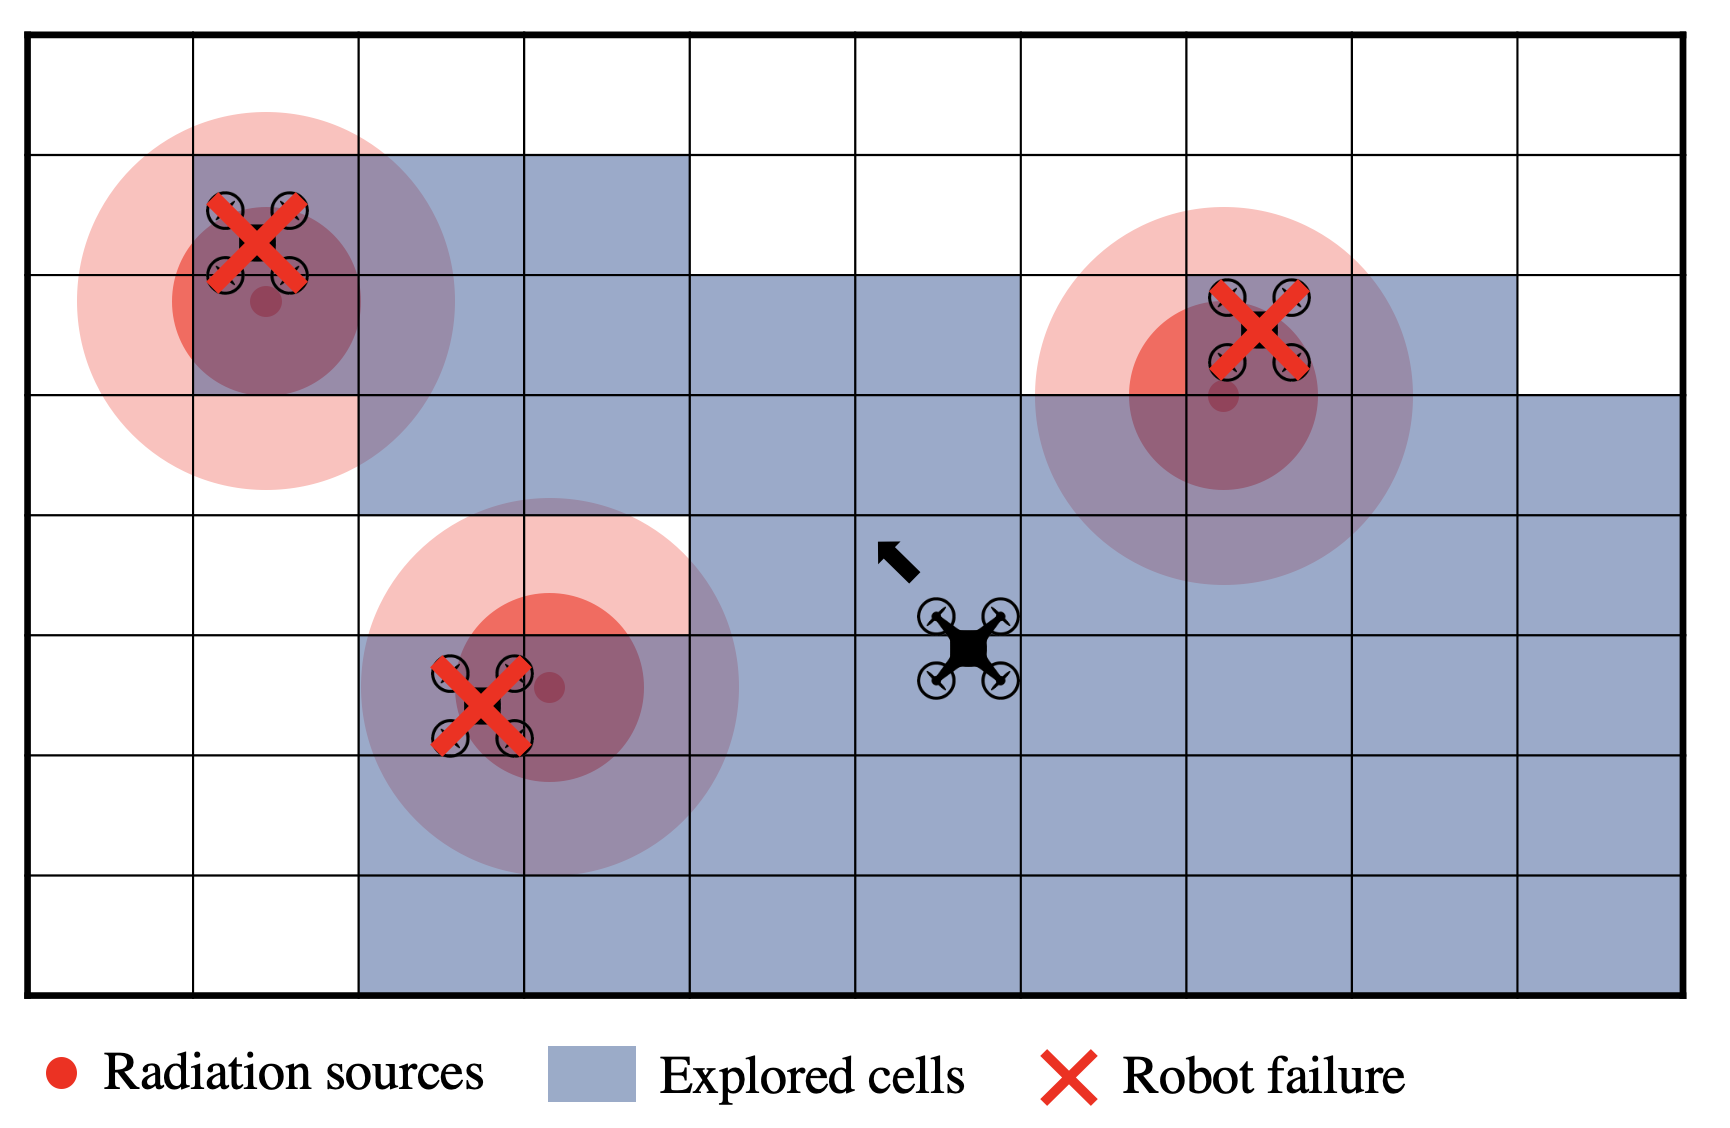
\includegraphics[width=\textwidth]{images/risk_unaware_a.png}
%          \caption{}
%          \label{risk_unaware_b}
%      \end{subfigure}
%         \caption{Exploration without risk awareness. Fig. \ref{risk_unaware_a}: Robots start exploring but are unable to sense environmental radiation. The only driving force of the algorithm is exploring new cells. Fig. \ref{risk_unaware_b}: Robots fail because they do not discriminate between safe and dangerous cells. Exploration is carried out fewer robots. Exploration efficiency drastically decreases and large areas of the environment remain uncovered.}
%         \label{risk_unaware}
% \end{figure*}

% \begin{figure*}[h]
%     \centering
%     % \begin{subfigure}{0.40\textwidth}
%     %      \centering
%     %      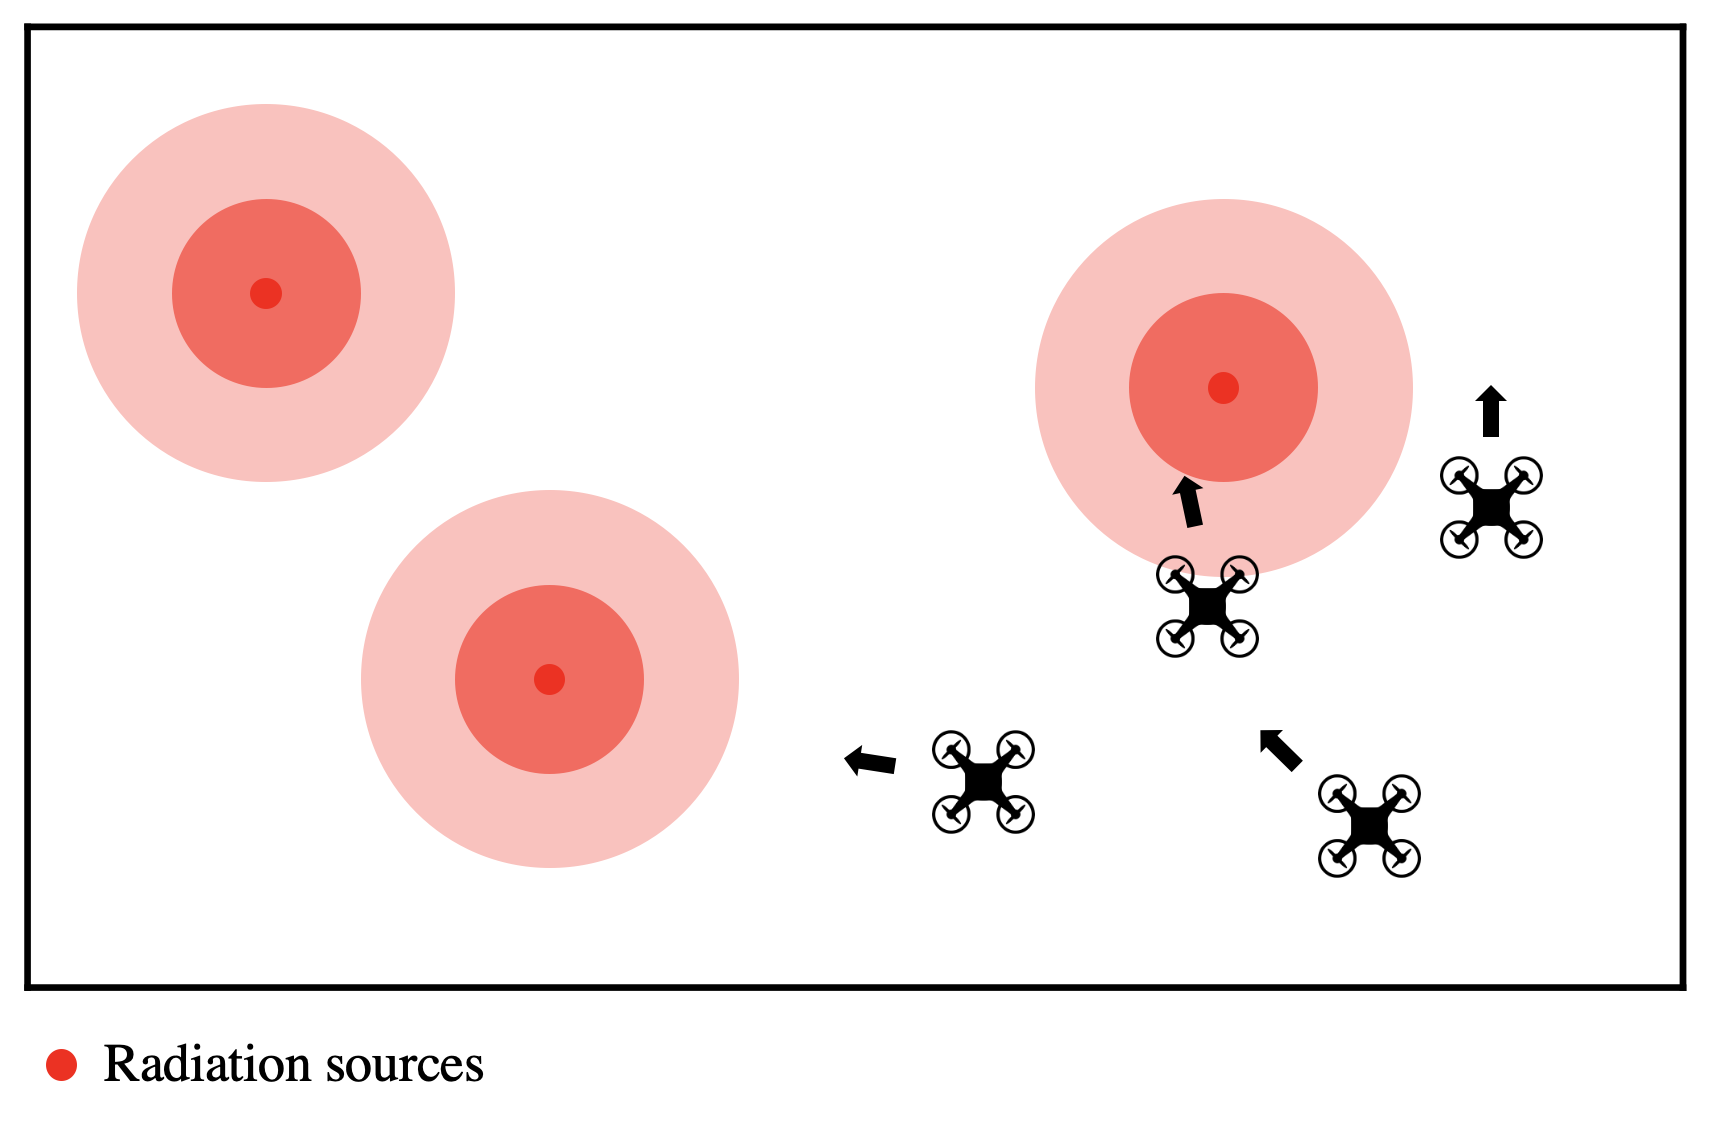
\includegraphics[width=\textwidth]{images/risk_aware_a.png}
%     %      \caption{}
%     %      \label{risk_aware_a}
%     % \end{subfigure}
%     % \hfill
%     \begin{subfigure}{0.30\textwidth}
%          \centering
%          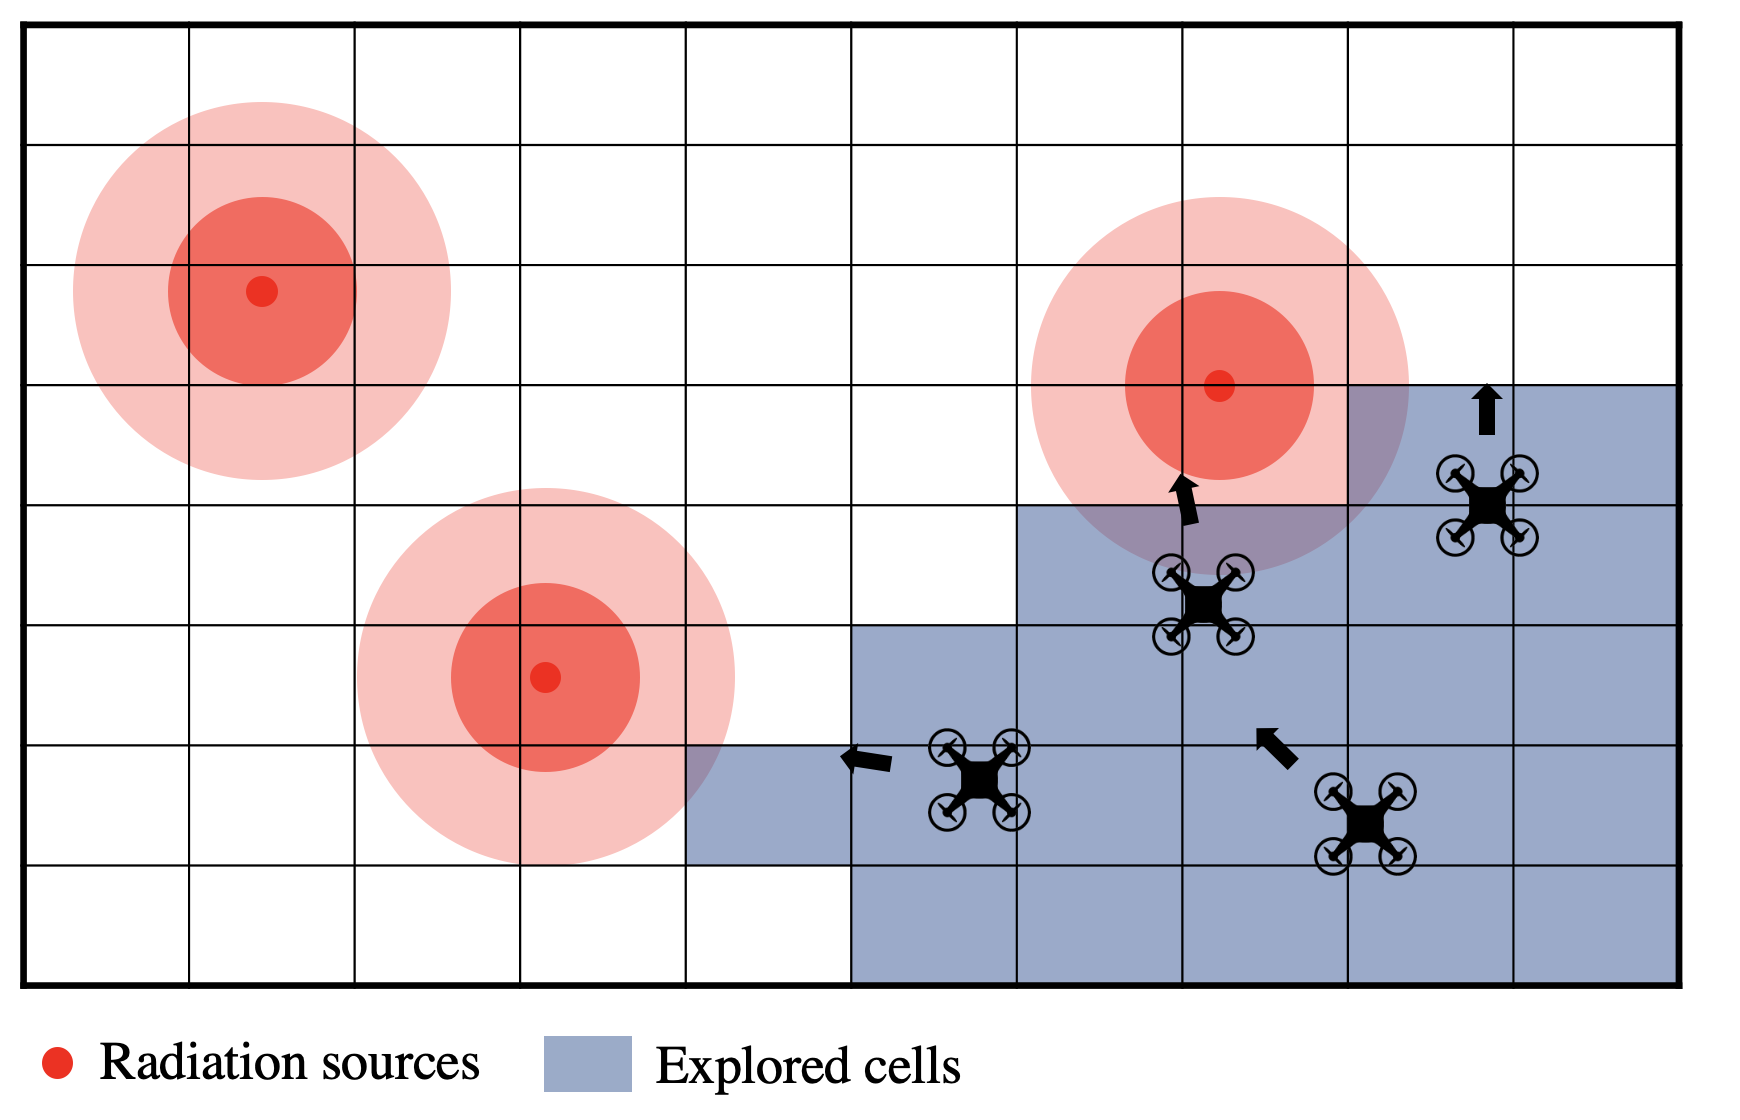
\includegraphics[width=\textwidth]{images/risk_aware_b.png}
%          \caption{}
%          \label{risk_aware_b}
%     \end{subfigure}
%     \hfill
%     \begin{subfigure}{0.30\textwidth}
%          \centering
%          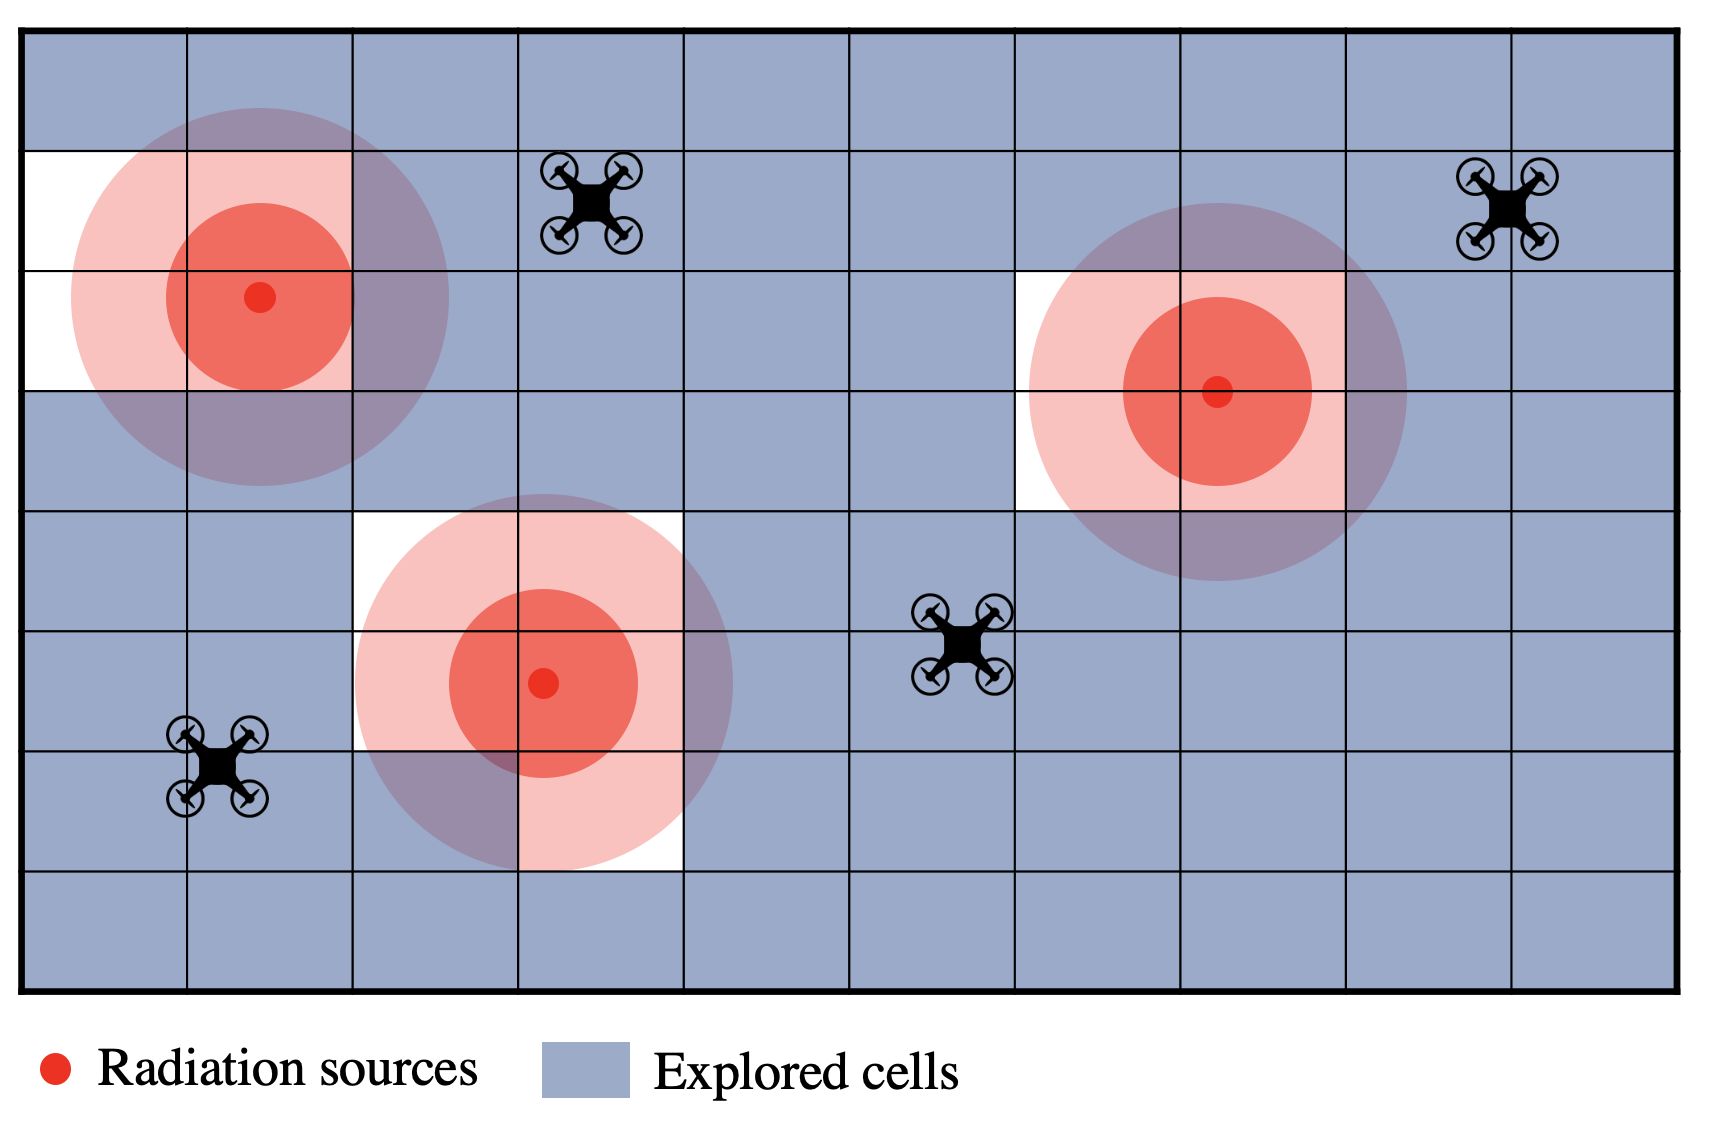
\includegraphics[width=\textwidth]{images/risk_aware_c.png}
%          \caption{}
%          \label{risk_aware_c}
%     \end{subfigure}
%     \hfill
%     \begin{subfigure}{0.30\textwidth}
%          \centering
%          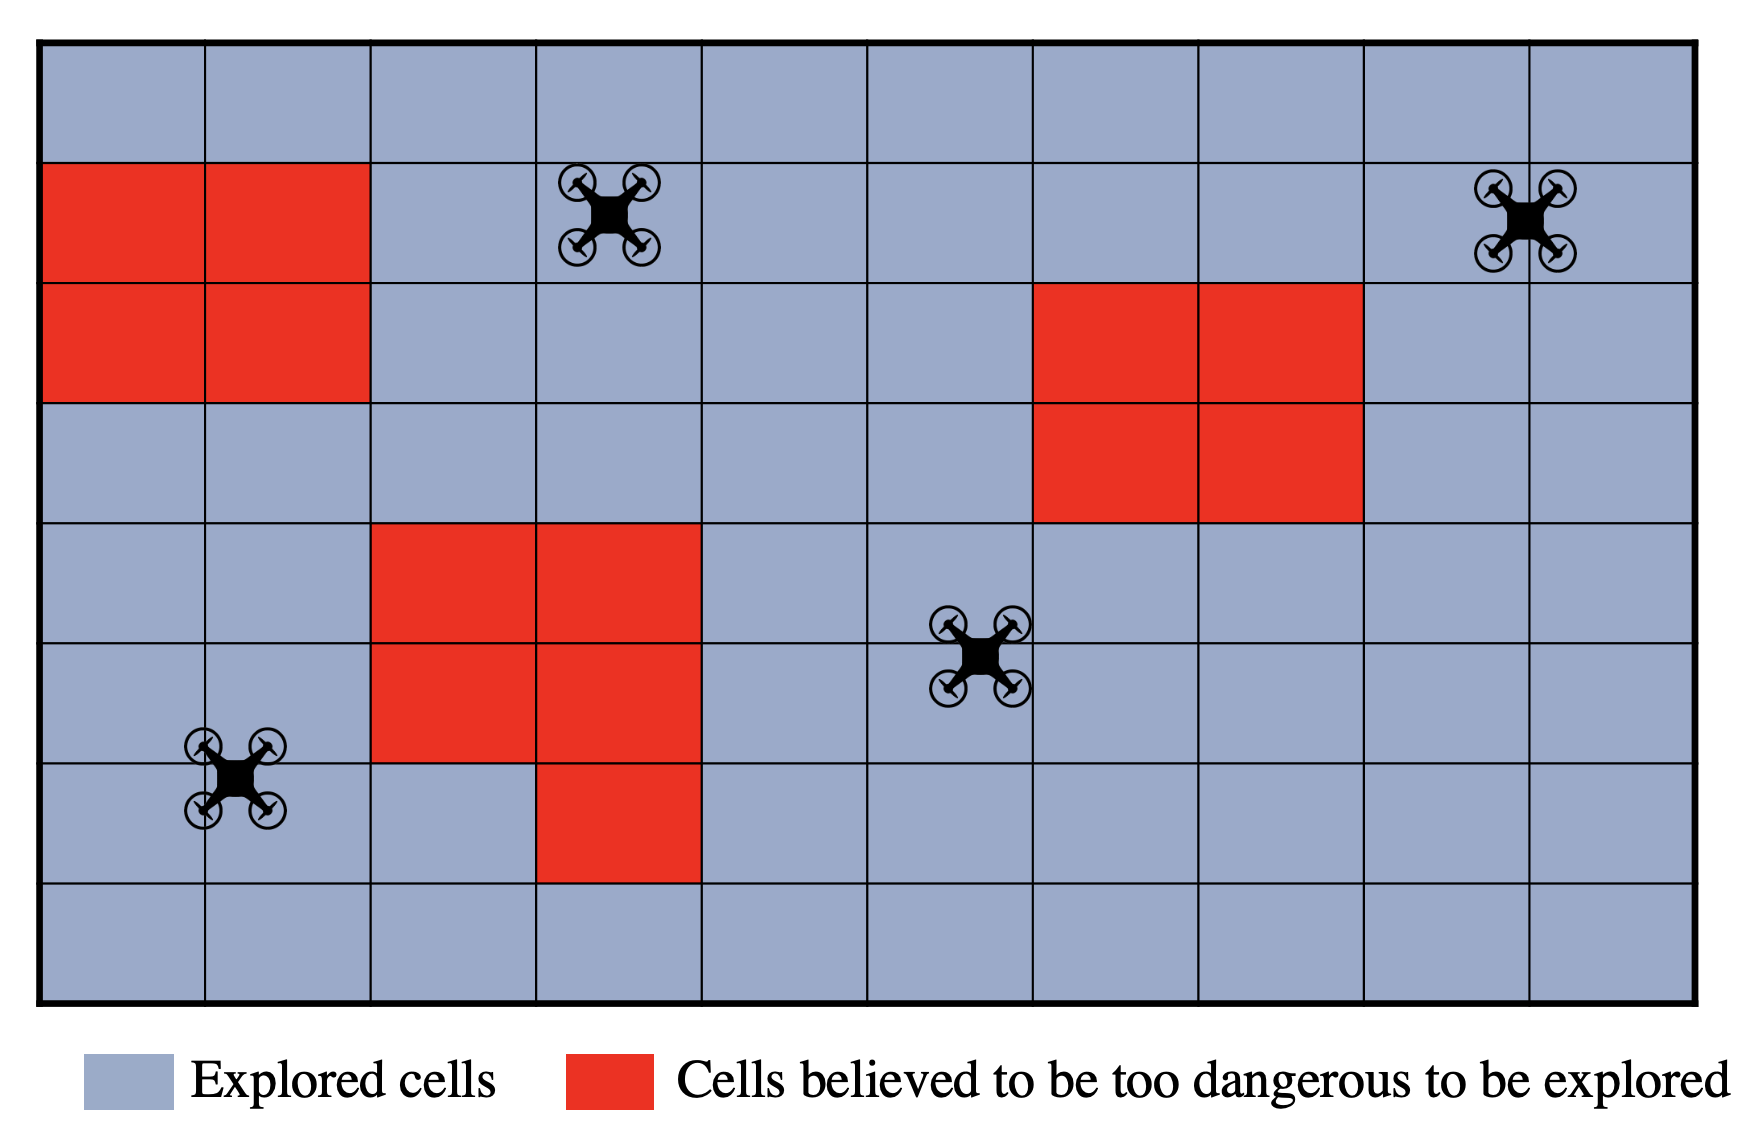
\includegraphics[width=\textwidth]{images/risk_aware_d.png}
%          \caption{}
%          \label{risk_aware_d}
%     \end{subfigure}
%         \caption{Risk aware exploration intuition. Fig. \ref{risk_aware_b}: Robots are dispatched in a hazardous environment and start exploring. When a new cell is explored by a robot, the sensed radiation is used to update the DBM. Fig. \ref{risk_aware_c}: The environment has been largely covered by the robots. Fig. \ref{risk_aware_d}: Only the cells believed to be too dangerous remain unexplored.}
%     \label{risk_aware}
% \end{figure*}

\subsection{Scalability}
\label{subsec:scalability}
To achieve scalability to a high number of agents and to large
environments, DORA-Explorer must have low communication and computational costs. Lowering the communication costs associated
with sharing the DBM can be done by using the virtual
stigmergy, which is designed to limit information exchange to read or
write operations only on the requested data. Because DORA-Explorer relies
solely on local information, the data transfer cost $D(A, \nu, E)$ for
an agent at a given time step is independent from the total number of
agents in $A$ and from the size of the environment $E$. For a
neighboring cell $\bm{n}_{i,j} \in \nu$, 2 stigmergy read operations
are needed per time step: one each to read $r(\bm{n}_{i,j})$ and
$\epsilon(\bm{n}_{i,j})$. In the same time step, the agent updates
$r(\bm{x}_i)$ and $\epsilon(\bm{x}_i)$ after it has moved to a new
location, which requires 2 stigmergy write operations. Each stigmergy
access requires only a few tens of bytes of data transfer for the key
and value. This mostly constant data quantity is represented as $d$,
we have $D(A, \nu, E) = 2d(|\nu| + 1)$. Similarly, the computational
cost $C(A, \nu, E)$ for the same agent at the same time step is kept
very low because of the reliance on local information only. Each time
step requires to compute 2 gradients, and referring to
\eqref{eq:gradient_risk}, \eqref{eq:gradient_exploration}, \eqref{eq:movement} and
\eqref{eq:control} we have that $C(A, \nu, E) = 12|\nu|+7$. The costs
related to $\bm{o}_i$ have been excluded from this analysis as
obstacle avoidance is not a critical part of DORA-Explorer. The step-wise communication
and computational costs for an agent are thus
both bounded by:

\begin{equation}
    D(A, \nu, E) \text{ and } C(A, \nu, E) \in \Theta(|\nu|)
    \label{eq:costs}
\end{equation}

Such low costs mean that DORA-Explorer should scale well to a large number of
robots and should enable real time computation on even very limited computational platforms.


\section{Simulations}
\subsection{Experimental setup}
\label{experimentSetup}

We tested our system through simulations in ARGoS
\cite{Pinciroli:SI2012}, which is an open-source physics-based
simulation environment designed for robotic swarms. The agents we used
in the simulation are KheperaIV robots 
\cite{kteam2021kheperaiv} programmed in Buzz \cite{pinciroliBuzz2016} to facilitate swarm
management and interaction. 

% These are small round robots (140mm of
% diameter) equipped with 8 infrared proximity sensors spread evenly
% around their frame to perform obstacle avoidance. The
% agents are programmed in Buzz to facilitate swarm
% management and interaction.

% \begin{figure}[h]
% 	\centering
%     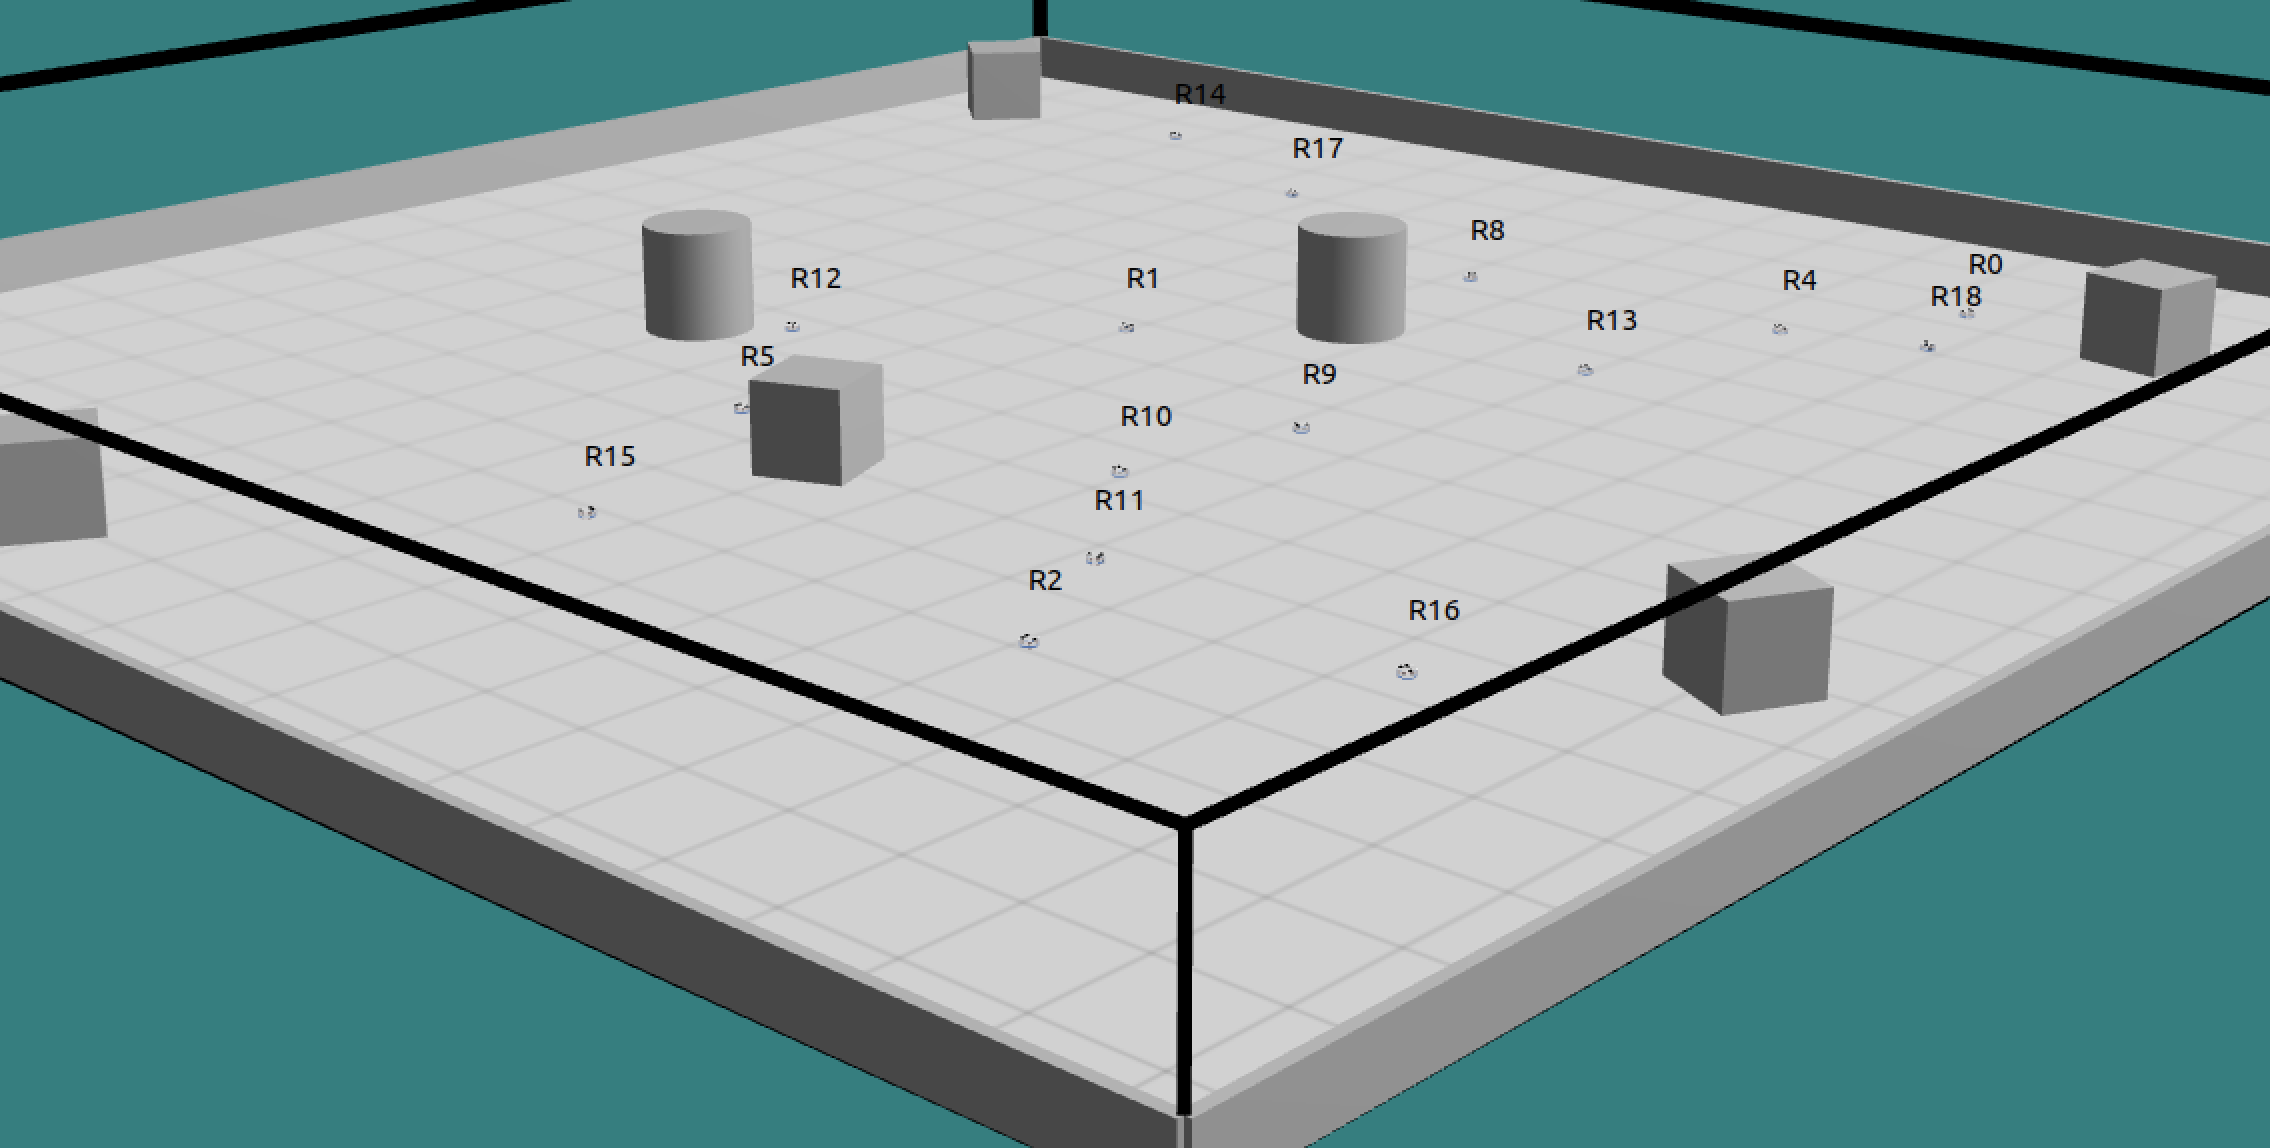
\includegraphics[width=0.95\columnwidth]{images/argos.png}
%     \caption{$400 \text{m}^2$ environment in the ARGoS simulator with 20 KheperaIV robots. Cylinders are radiation sources and boxes are random obstacles.}
%     \label{argos}
% \end{figure}

We deployed a set of N = \{10, 15, 20\} robots in a simulated
environment of 20x20m with set of 2 radiation sources. The environment is discretized into 400 cells, where each cell of the grid is 1x1m large. The robots'
initial positions are chosen randomly. We arbitrarily set $\lambda$ from
\eqref{eq:radiation} to be 5 as it was providing an adequate decay speed in relation with the size of our environment: The robots would generally fail in a 3m radius around the radiation sources. The speed constant $k$ from \eqref{eq:control} is set to
$20$ to match the maximal speed of the KheperaIV robots. Because no information gain can be achieved by a failed robot, failure must be avoided. This
leads to choosing $\alpha >= \beta$ in \eqref{eq:control}. For our
experiments, we set $\alpha=2, \beta=1$ and $\gamma=1$. The robots are
all given a random initial orientation. Radiation sensing is emulated
by an ARGoS controller reading the randomly generated radiation
sources. Failures are randomly triggered by using \eqref{eq:failure}:
if $f_i=1$, the robot stops exploring. We added 5 randomly distributed
0.8m x 0.8m obstacles to verify the robot's ability to
perform exploration even in cluttered environments.

% \begin{figure*}
%     \centering
%     \begin{subfigure}{0.32\textwidth}
%         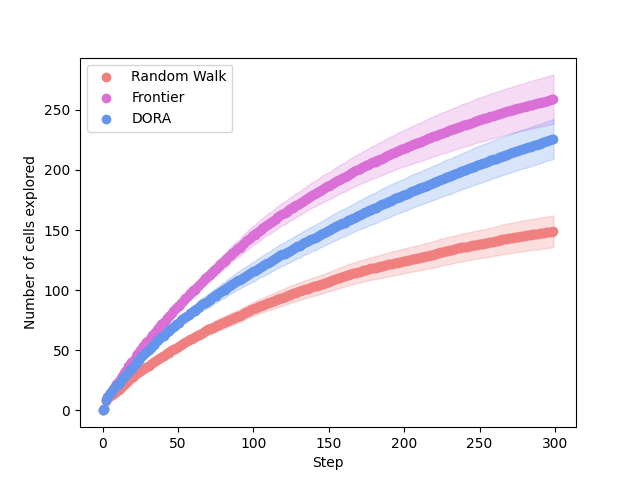
\includegraphics[width=\textwidth]{images/explored_10.png}
%         \caption{N=10 robots}
%         \label{results:explored10}
%     \end{subfigure}
%     \begin{subfigure}{0.32\textwidth}
%         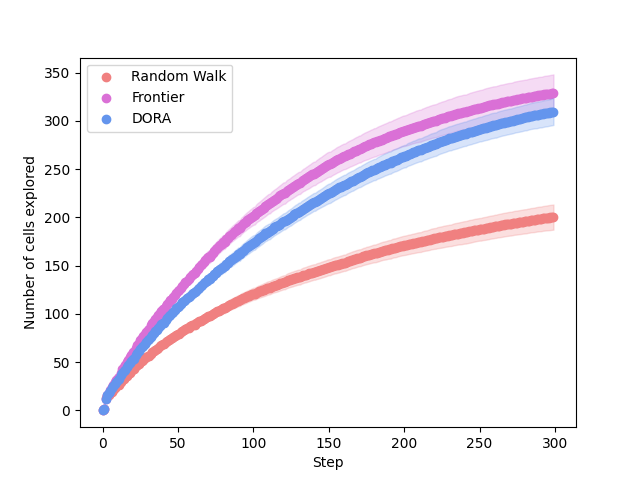
\includegraphics[width=\textwidth]{images/explored_15.png}
%         \caption{N=15 robots}
%         \label{results:explored15}
%     \end{subfigure}
%     \begin{subfigure}{0.32\textwidth}
%         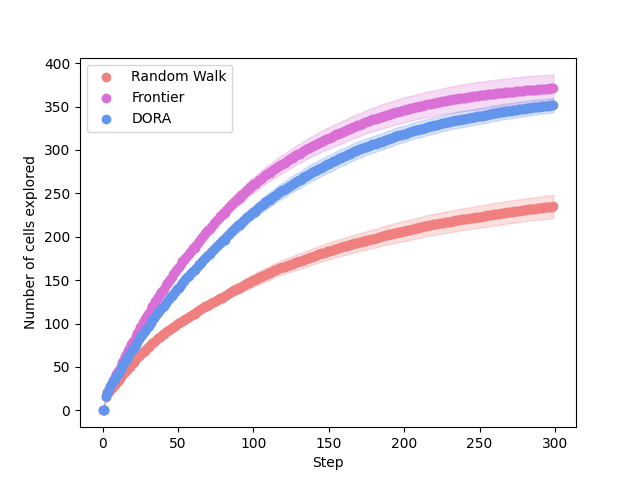
\includegraphics[width=\textwidth]{images/explored_20.png}
%         \caption{N=20 robots}
%         \label{results:explored20}
%     \end{subfigure}
%     \caption{Performance comparison of DORA-Explorer, FBE and random walk for number of explored cells over time.}
    
% \end{figure*}

% \begin{figure*}
%     \centering
%     \begin{subfigure}{0.32\textwidth}
%         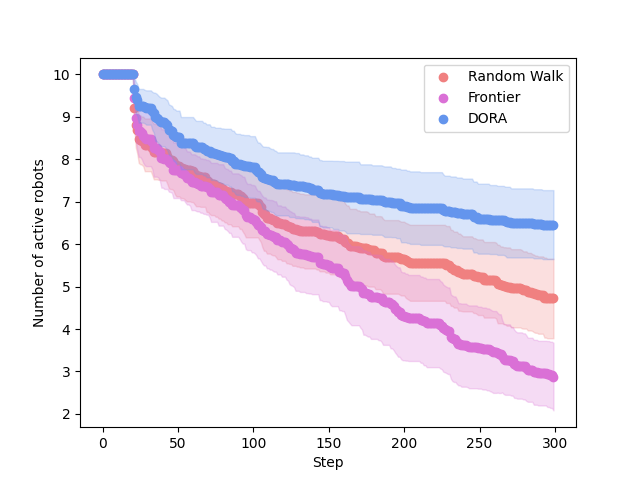
\includegraphics[width=\textwidth]{images/activerobots_10.png}
%         \caption{N=10 robots}
%         \label{results:failures10}
%     \end{subfigure}
%     \begin{subfigure}{0.32\textwidth}
%         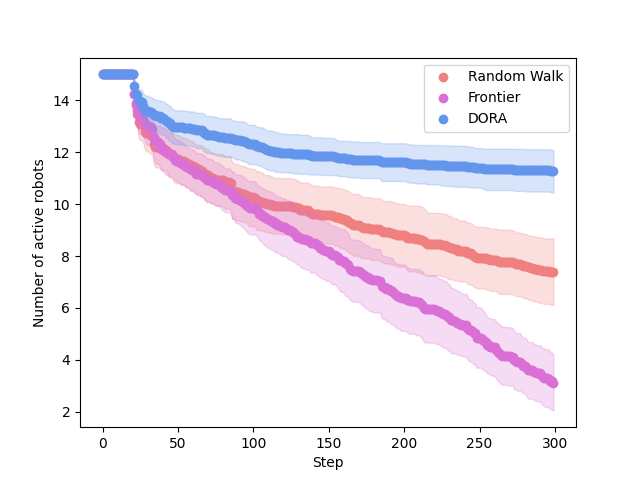
\includegraphics[width=\textwidth]{images/activerobots_15.png}
%         \caption{N=15 robots}
%         \label{results:failures15}
%     \end{subfigure}
%     \begin{subfigure}{0.32\textwidth}
%         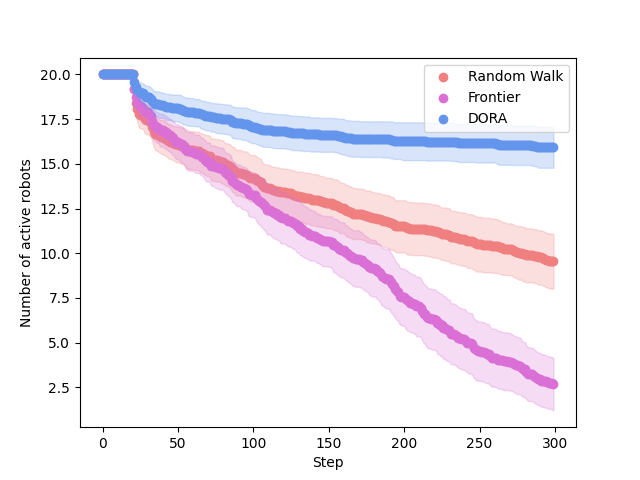
\includegraphics[width=\textwidth]{images/activerobots_20.png}
%         \caption{N=20 robots}
%         \label{results:failures20}
%     \end{subfigure}
%     \caption{Performance comparison of DORA-Explorer, FBE and random walk for number of active robots over time.}
% \end{figure*}



We performed 50 simulation runs over 300 steps of the DORA-Explorer
algorithm. Each time step lasts 0.8s. To assess DORA-Explorer's performance, we compare it to the results
obtained by a random walk algorithm and by a FBE algorithm. The
latter's key principle is to assign one of three states (explored,
frontier, unexplored) to the cells constituting the environment and to
coordinate the robots to explore the regions near the frontier. To
implement it, we adapted the algorithm from
\cite{yamauchi1998frontier} by having the robots share an exploration
map through a virtual stigmergy. The comparison with frontier exploration is
particularly relevant because it allows us to gain insights on our
algorithm performance in terms of terrain coverage compared to an
algorithm which was specifically designed to maximize this
objective. We also compare DORA-Explorer with a random walk algorithm as a
baseline it absolutely needs to outperform. These two baselines are
commonly used for the exploration of unknown environments in the field
of swarm robotics. They do not take risk into account, but to the best
of our knowledge, no other existing swarm exploration strategy does. To address this issue, we could have modified the baselines to take risk into account, but chose against it. Adding risk thresholds for movement could be considered. However, if the robots find themselves in radiation hotspots, they might remain stuck in these locations because all surrounding cells will a have similar/equal risk which is too high to allow movement, resulting in fatal stagnation. 

% Obstacle avoidance algorithms could have also been adapted to a risk avoidance context and serve as a baseline for DORA-Explorer. However, taking account of varying levels of risk would have been challenging. Again, it is hard to determine the threshold on risk level after which a cell should be considered as containing an obstacle.

% For the FBE method, a possibility would have been to treat radiation sources as obstacles and use an obstacle avoidance mechanism to stay away from them.
% However, there are two issues with this. First, these algorithms mostly focus on avoiding one obstacle at a time (the closest one), and therefore do not consider the effect of combined obstacles. This would not make sense anyway: two obstacles cannot be at the same location, while radiation sources can have a combined effect in one location. Second, these algorithms usually detect the presence of an obstacle in a binary way and are thus ill-suited for the presence of a gradual risk.

The first metric used to assess the validity of our approach is the
number of robots which remain active (not failed) over time. This is
perhaps the most important metric because it shows how well DORA-Explorer
performs in terms of risk avoidance, i.e. its main objective. The
second metric used to evaluate the algorithms is the total number of
cells explored by the swarm. This allows us to evaluate how well our
algorithm performs in its objective of maximizing information gain and
to verify that avoiding risk does not impact too much the exploration
performance. The third metric we studied is the communication costs of
the algorithms, measured in KB of data transmitted per robot at
each time step. We included this in our analysis to examine if
the algorithms can scale to large number of robots. We also ran simulations to study the impact of the parameters $\alpha$ and $\beta$ from (\ref{eq:movement}). 


\subsection{Results}

\begin{figure}[]
    \centering
    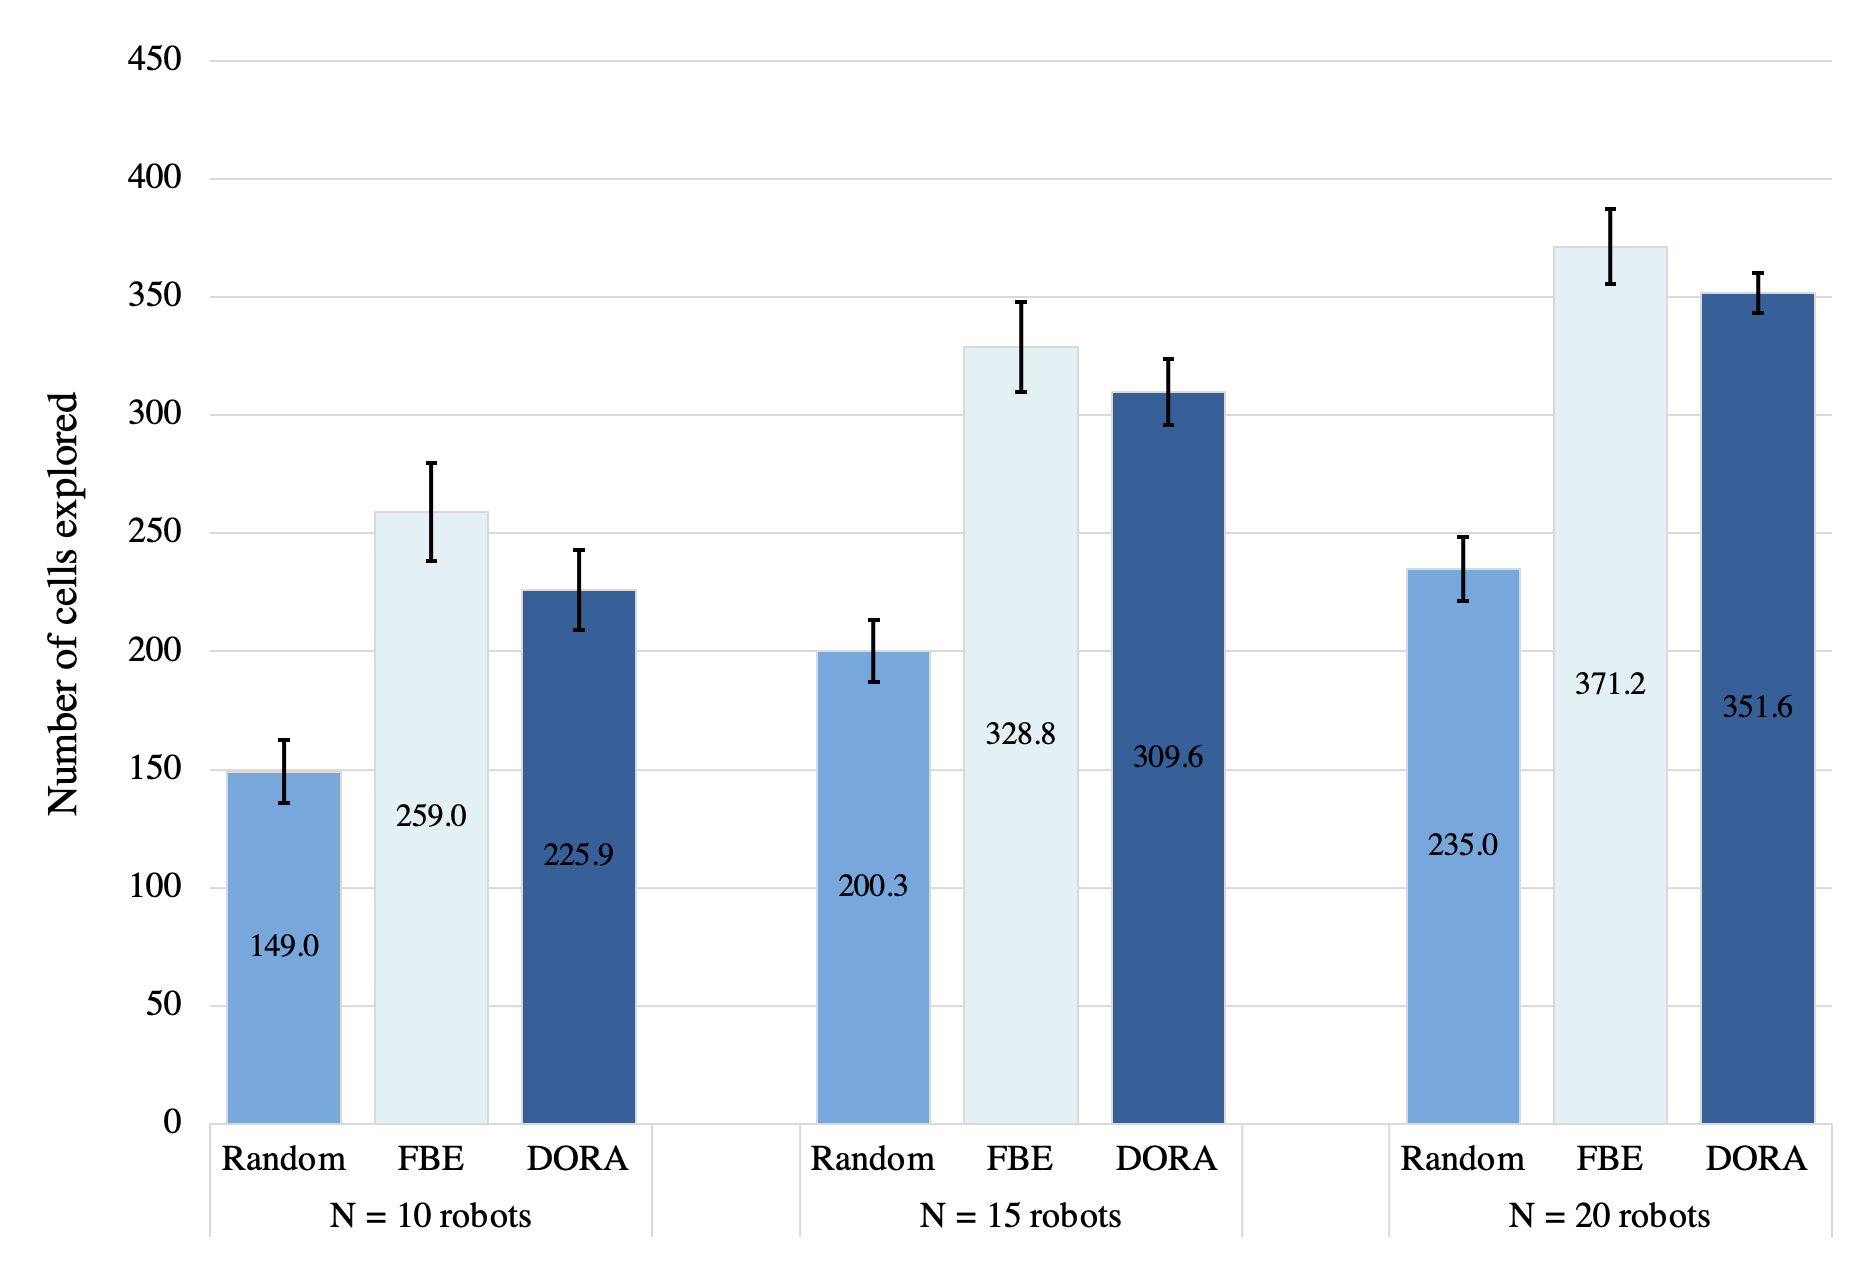
\includegraphics[width=1\columnwidth]{images/cell_explored.png}
    \caption{Performance comparison of DORA-Explorer, FBE and random walk for number of explored cells at the end of the simulation.}
    \label{results:exploration}
\end{figure}

\begin{figure}[]
    \centering
    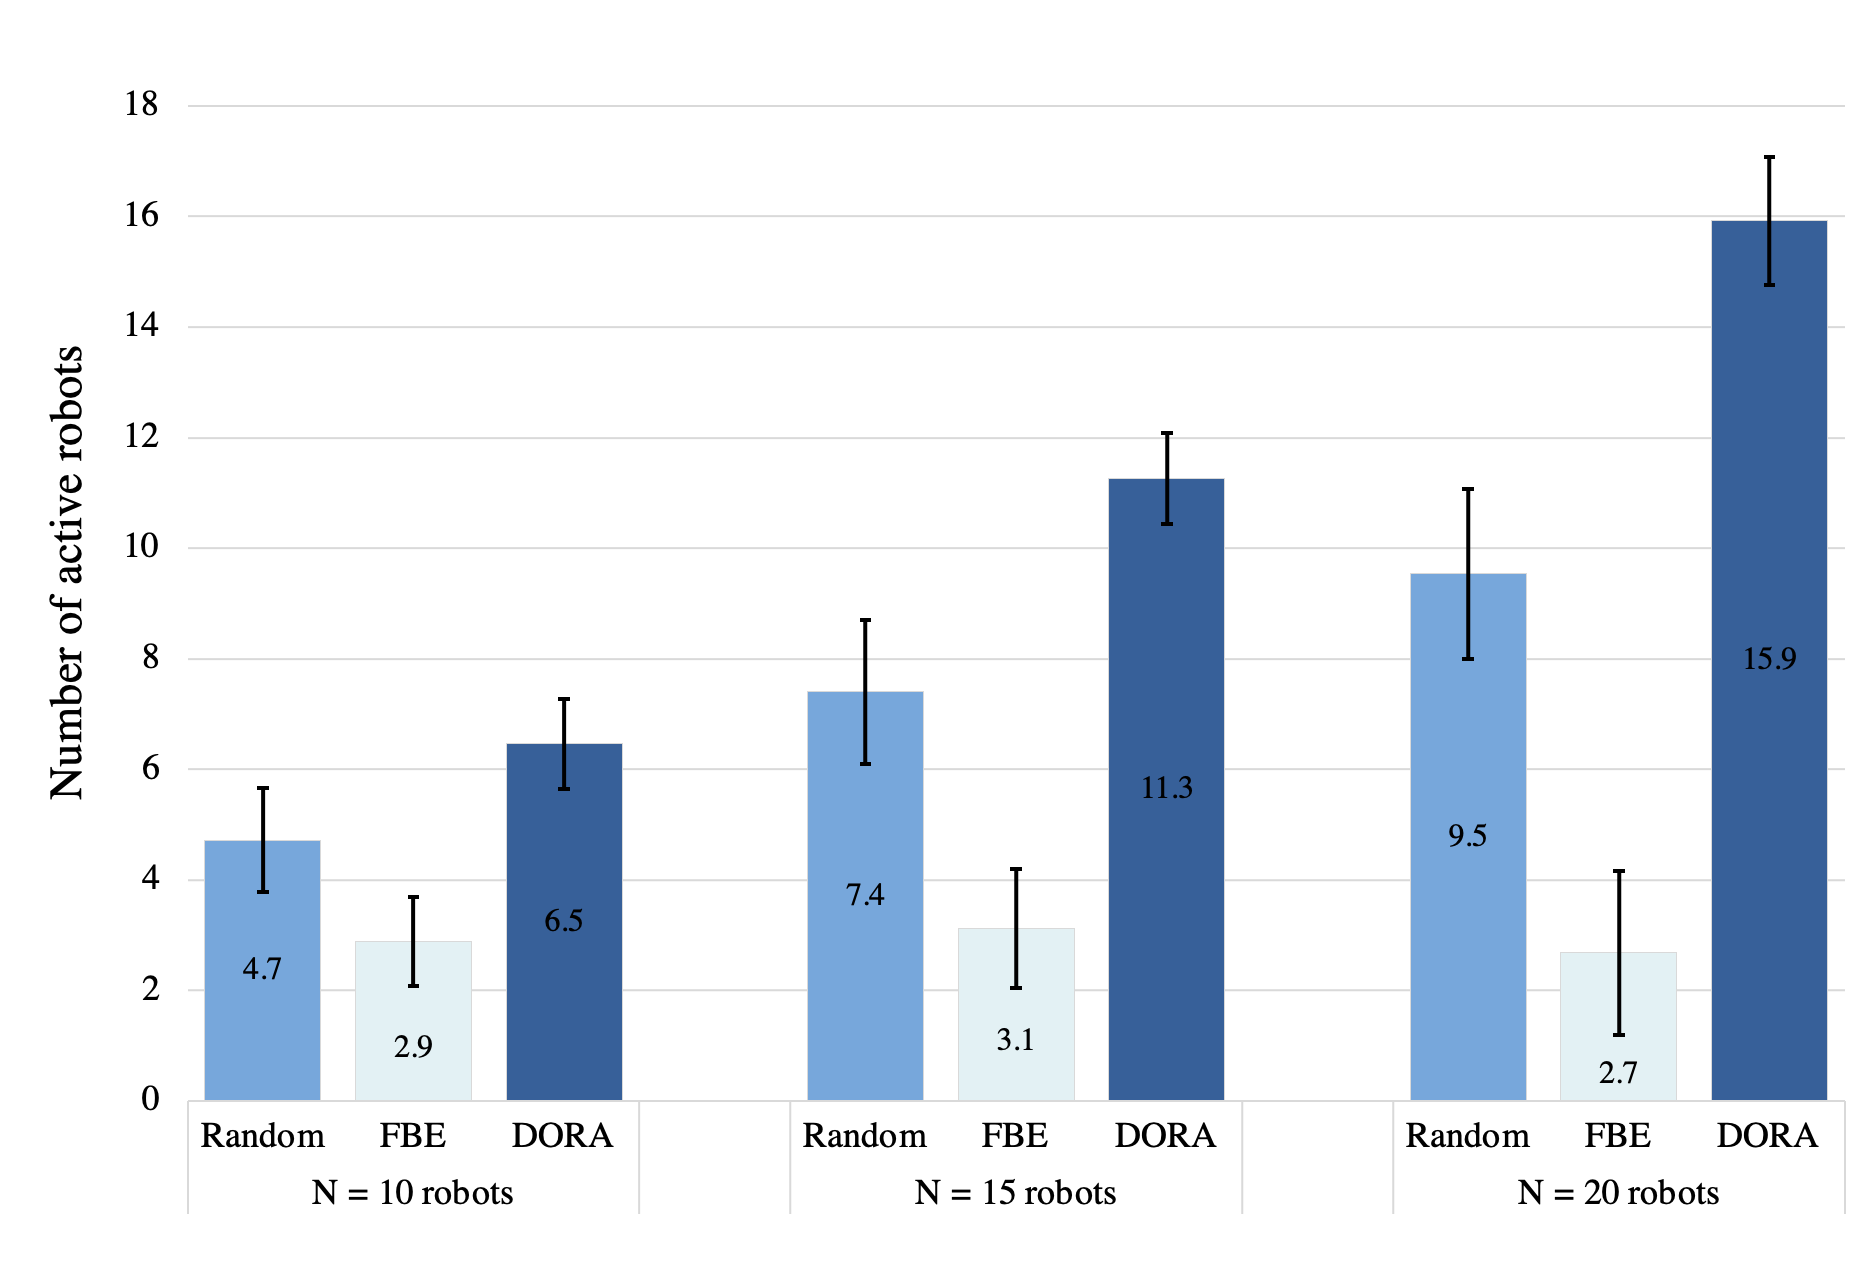
\includegraphics[width=1\columnwidth]{images/active_robot.png}
    \caption{Performance comparison of DORA-Explorer, FBE and random walk for number of active robots at the end of the simulation.}
    \label{results:active}
\end{figure}


The following results are an average of the 50 simulation runs of each algorithm. Results from Fig. \ref{results:exploration} show that FBE
achieves slightly higher exploration coverage than DORA-Explorer, but this
gap in performance decreases as the number of robots increases. This
is an expected result, because DORA-Explorer's main goal is not to achieve
maximal coverage at all costs, unlike FBE. Both FBE and DORA-Explorer clearly
outperform the random walk algorithm. The other trend is that adding
more robots to the swarm results in a higher
number of cells being explored for all three algorithms after 300
steps. This shows that DORA-Explorer scales well to large number of robots, and even gains in performance when swarm size increases, which is in line
with the benefits associated with swarm algorithms. In terms of avoiding failures, DORA-Explorer unsurprisingly outperforms both
FBE and the random walk, as it is its main purpose. This is shown in
Fig. \ref{results:active}, where DORA-Explorer exhibits a higher level of active
robots at the end of the simulation runs, with this difference only increasing with larger
swarm sizes. For all values of N, there are few
survivors for FBE, and random walks perform only slightly better, while DORA-Explorer keeps most robots alive, achieving its objective.


Fig. \ref{results:belief} shows the DBMs obtained at the end of an
arbitrarily selected simulation where N = 20 for each algorithm.  In
other words, it represents which cells were explored by each algorithm
and the sensed radiation intensity associated with them for one specific run. 

\begin{figure}[h]
    \centering
    \subfigure[]
        {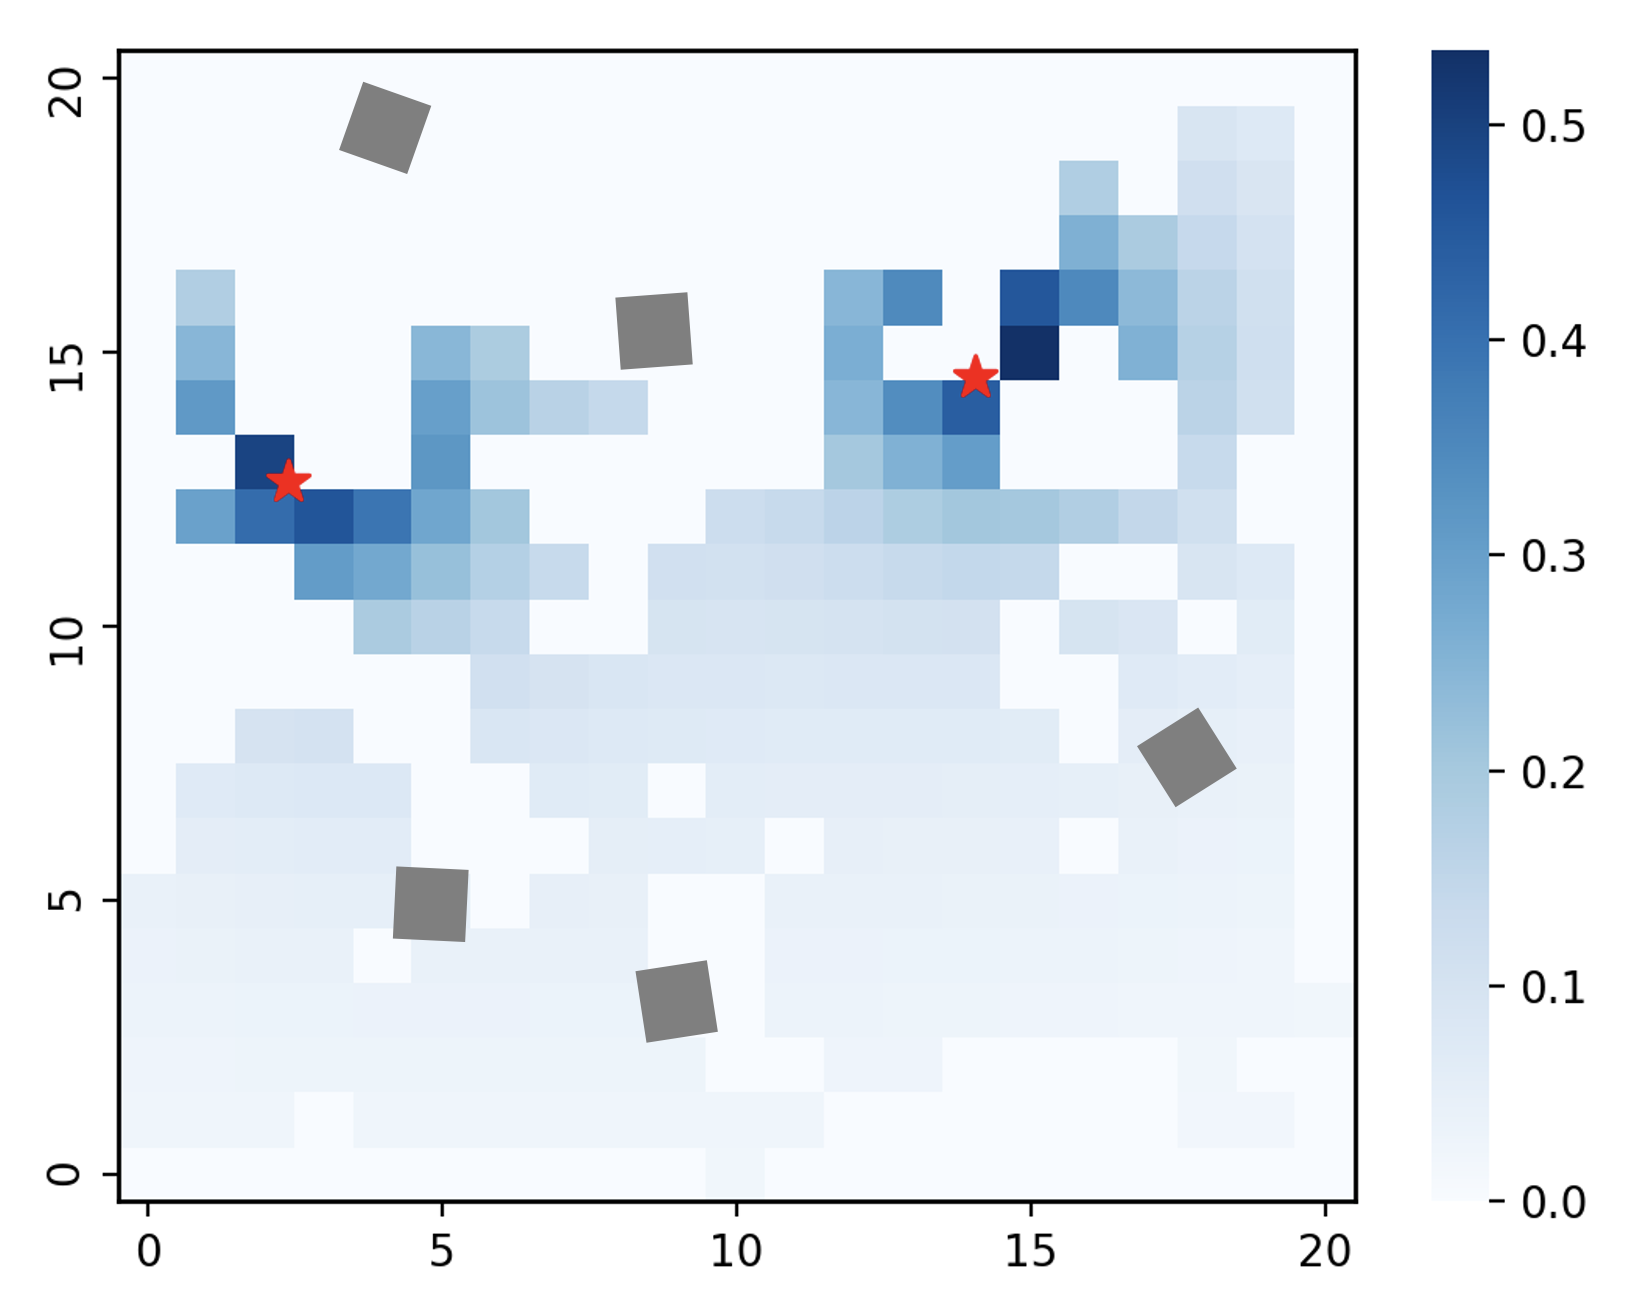
\includegraphics[width=0.47\textwidth]{images/heatmap_random.png}
        \label{results:beliefrandom}
        }
    \subfigure[]
        {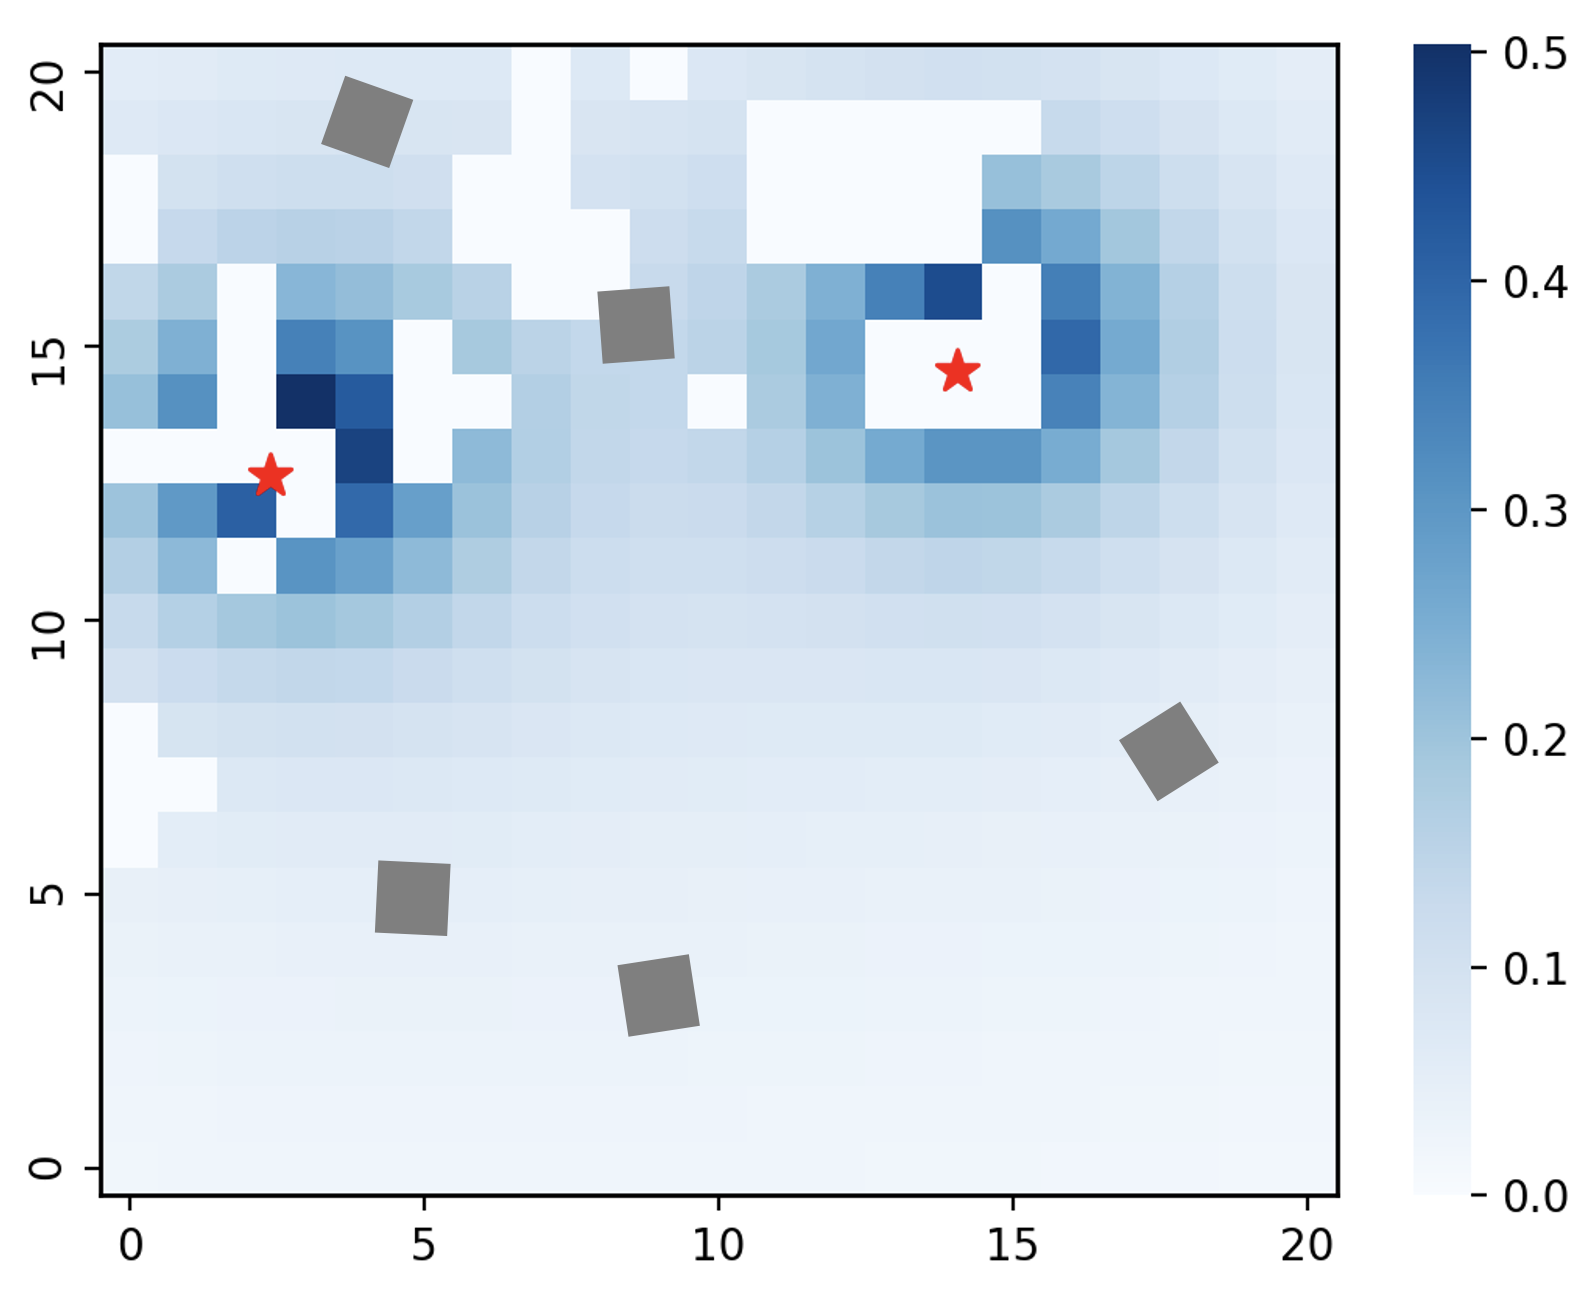
\includegraphics[width=0.47\textwidth]{images/heatmap_frontier.png}
        \label{results:belieffrontier}
        }
    \subfigure[]
        {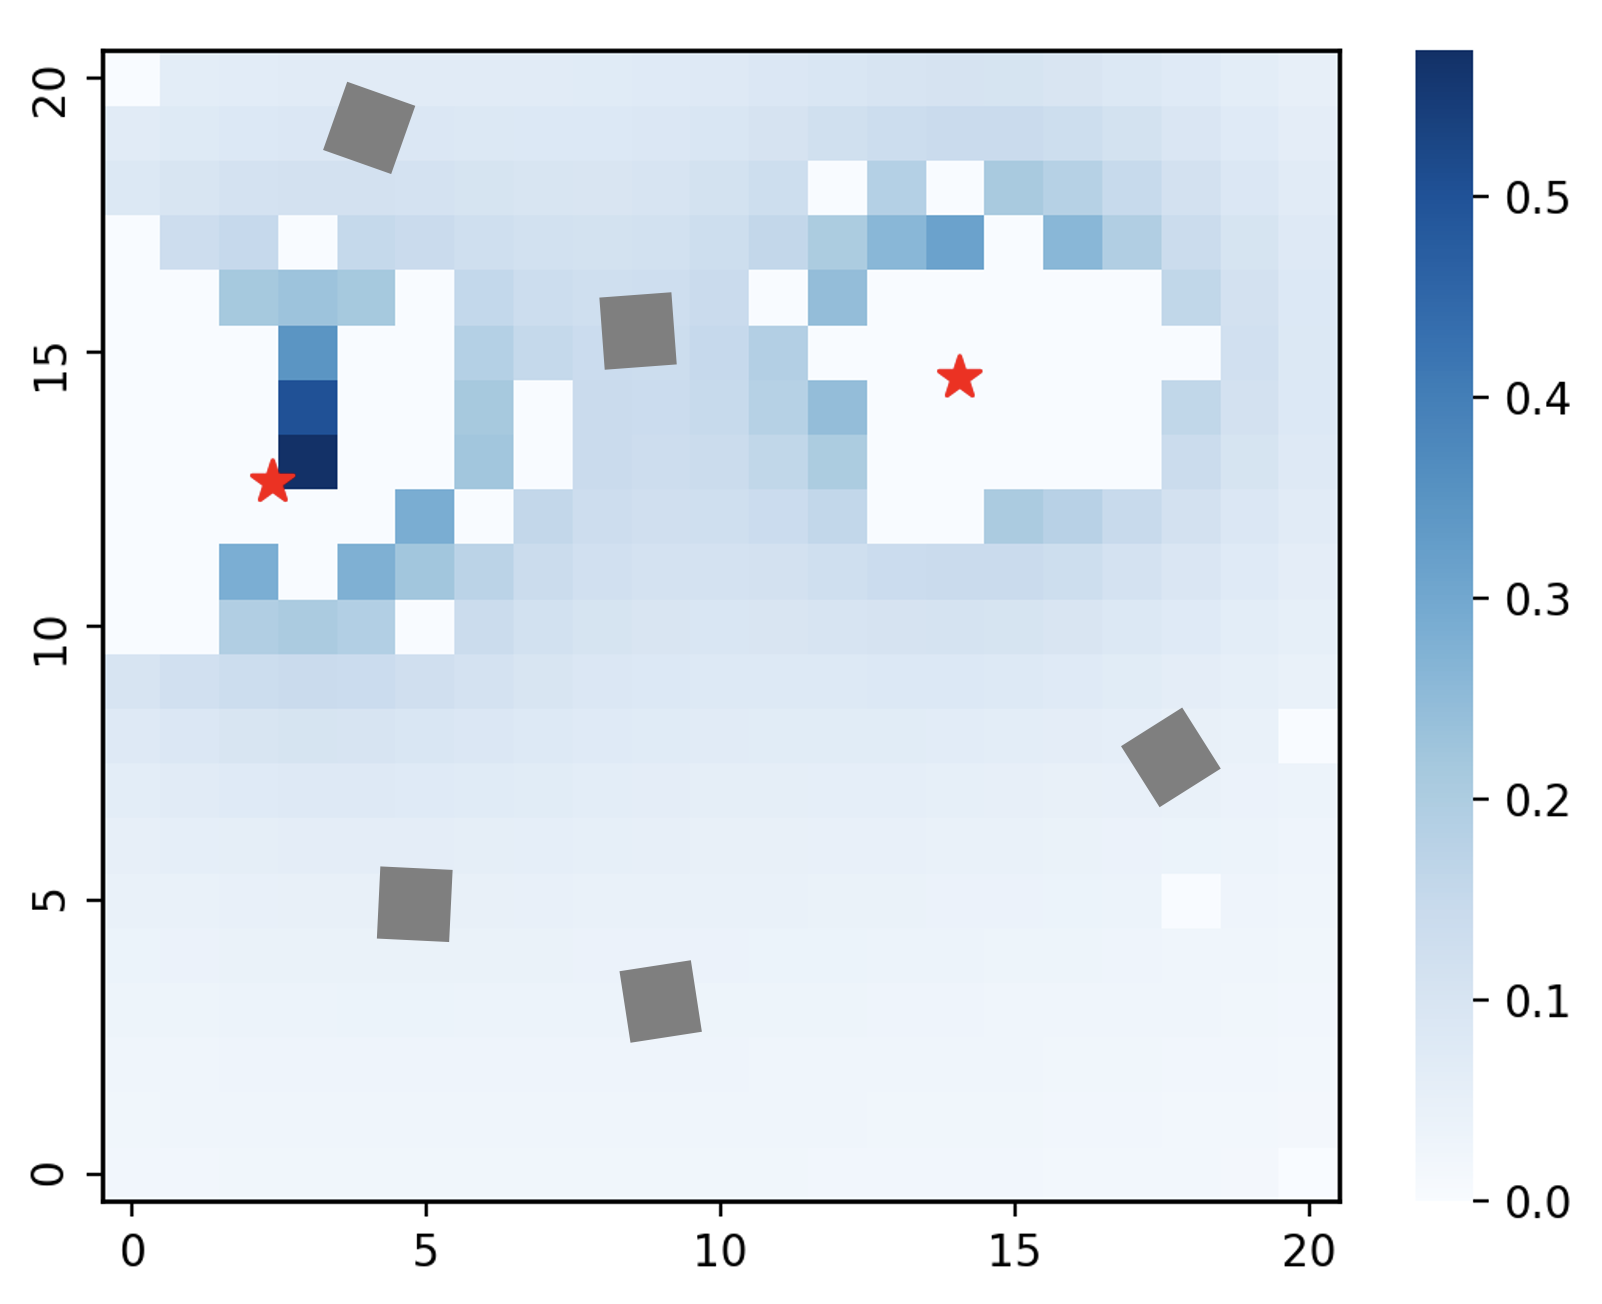
\includegraphics[width=0.47\textwidth]{images/heatmap_dora.png}
        \label{results:beliefdora}
        }
    \caption{(a) Random walk (b) FBE (c) DORA-Explorer. Radiation belief maps of the 20m x 20m environment for each exploration algorithm of one specific simulation. Blank cells are unvisited areas, red stars are the point radiation sources and grey squares are the randomly generated obstacles.}
    \label{results:belief}
\end{figure}

% \begin{figure}[h]
%     \centering
%     \begin{subfigure}{0.49\textwidth}
%         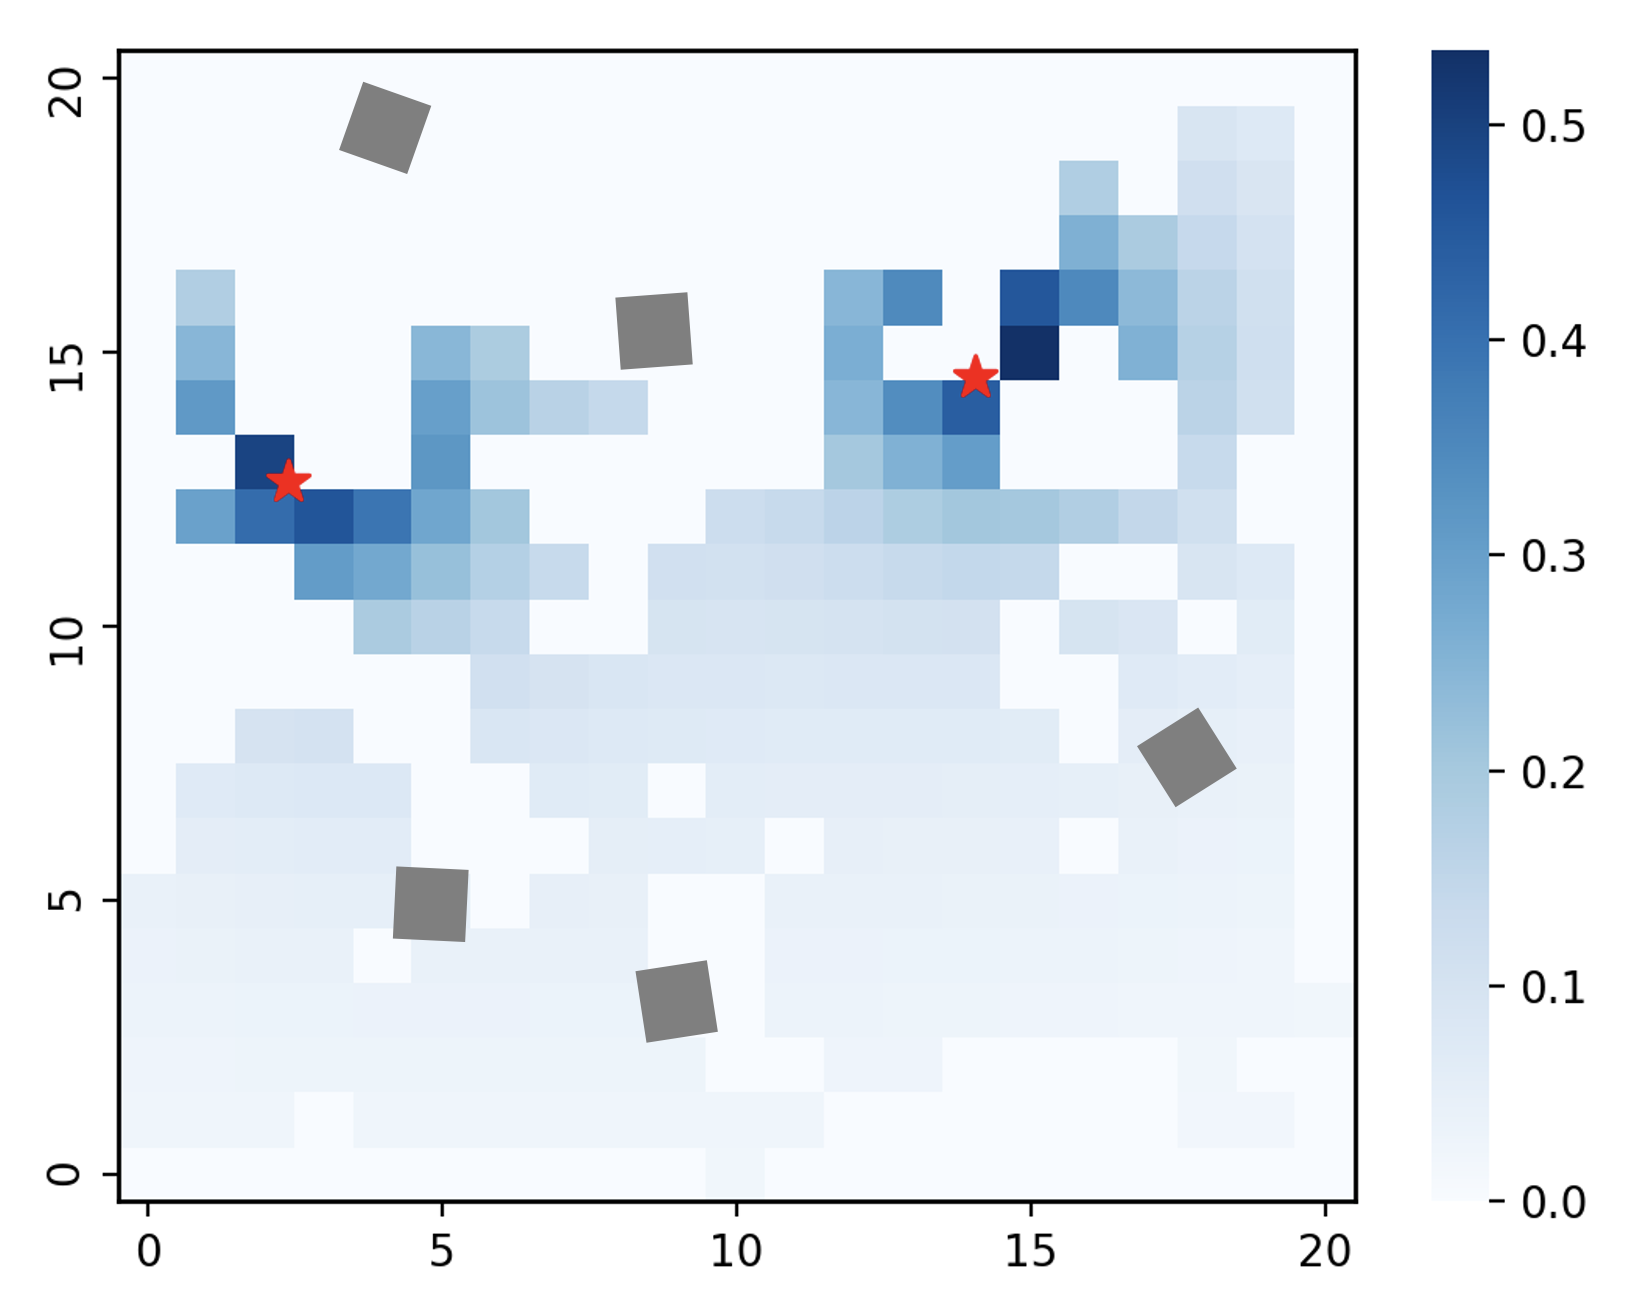
\includegraphics[width=\textwidth]{images/heatmap_random.png}
%         \caption{Random walk}
%         \label{results:beliefrandom}
%     \end{subfigure}
%     \begin{subfigure}{0.49\textwidth}
%         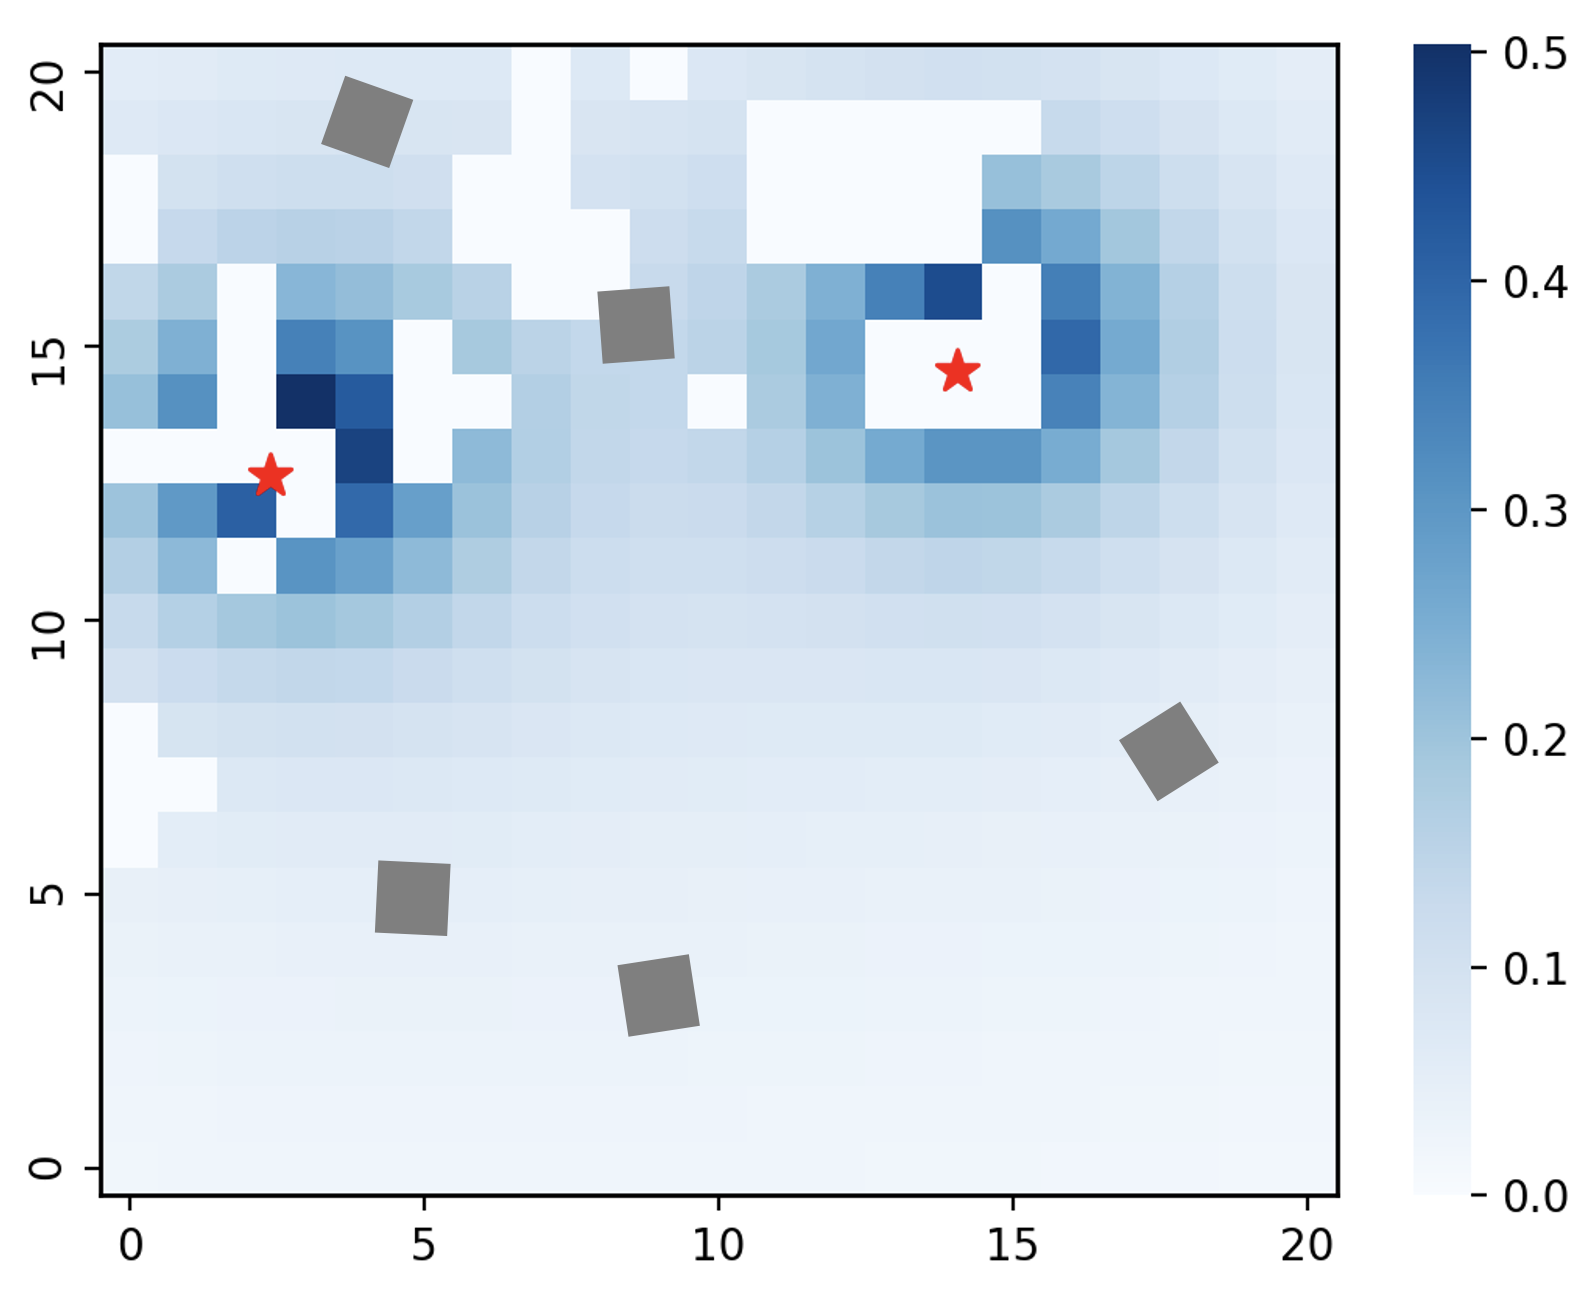
\includegraphics[width=\textwidth]{images/heatmap_frontier.png}
%         \caption{FBE}
%         \label{results:belieffrontier}
%     \end{subfigure}
%     \begin{subfigure}{0.49\textwidth}
%         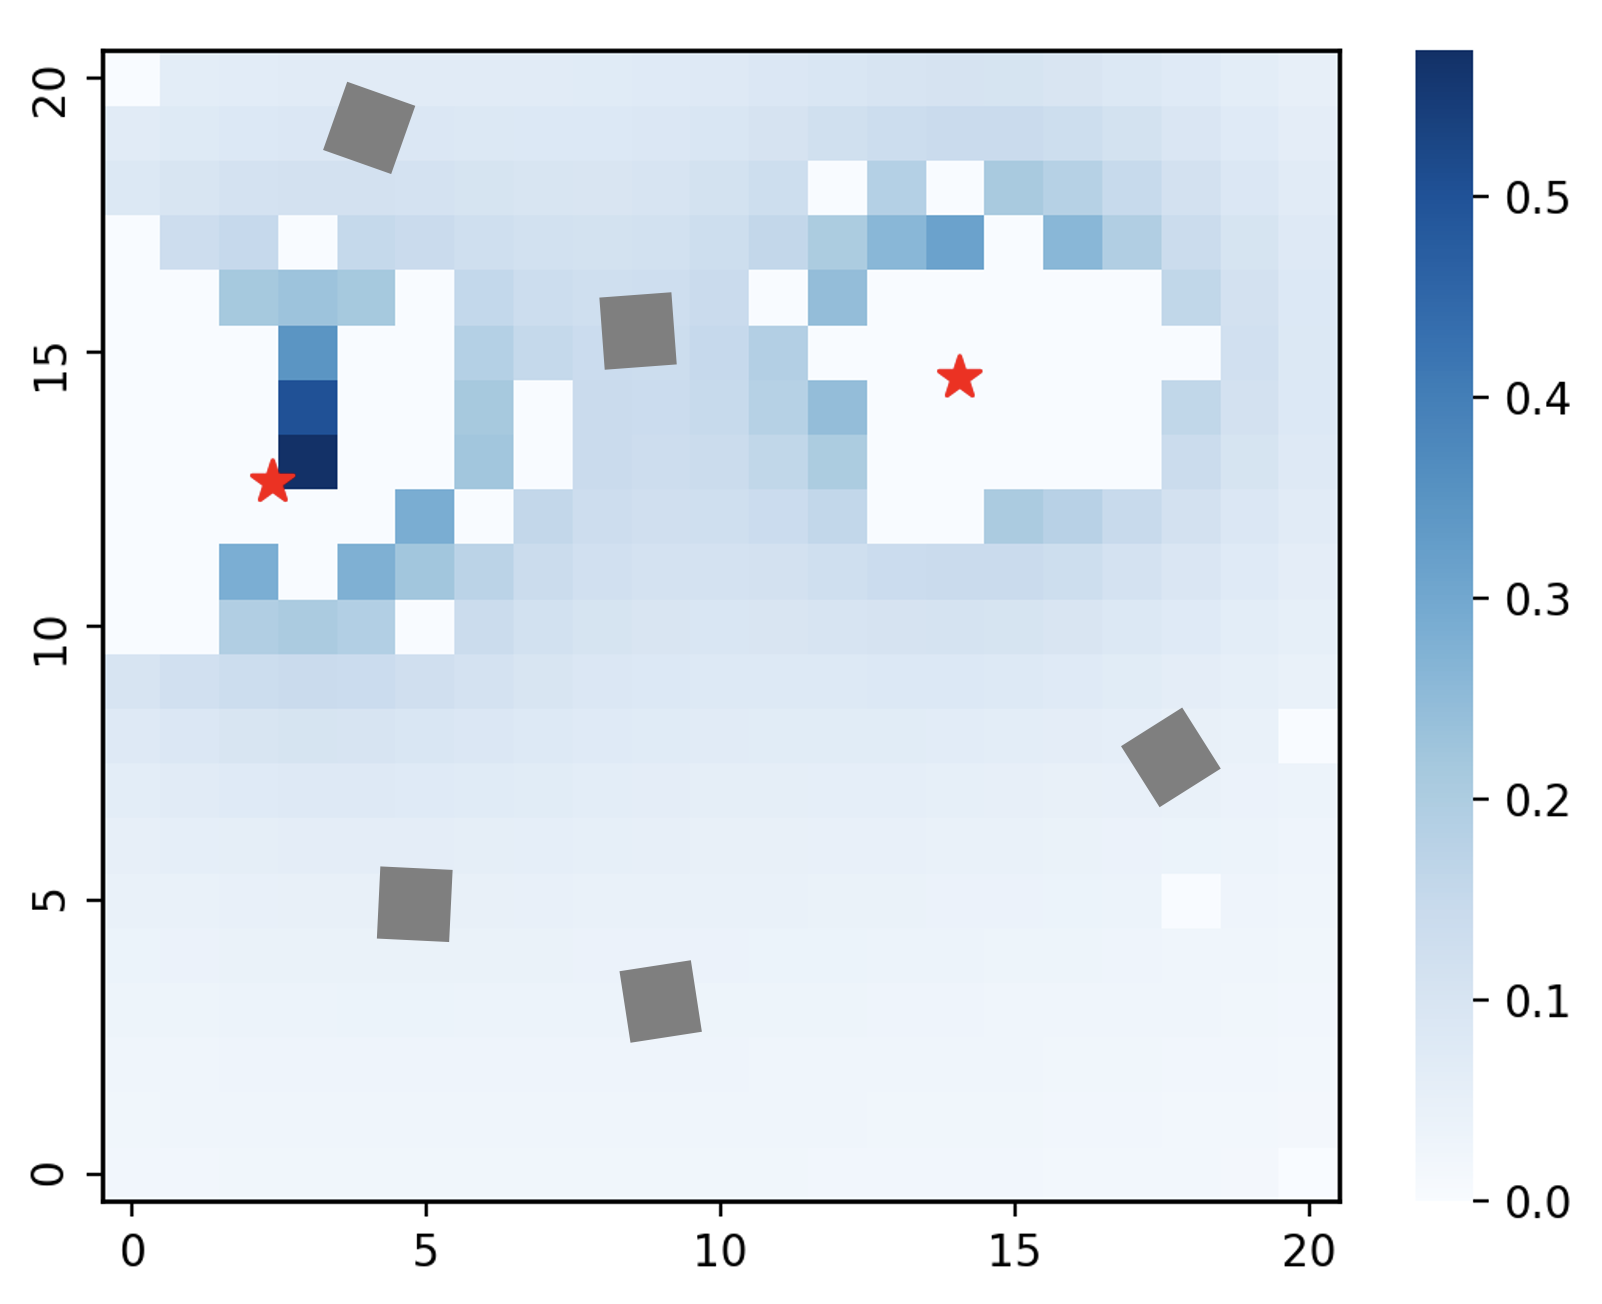
\includegraphics[width=\textwidth]{images/heatmap_dora.png}
%         \caption{DORA-Explorer}
%         \label{results:beliefdora}
%     \end{subfigure}
%     \caption{Radiation belief maps of the 20m x 20m environment for each exploration algorithm of one specific simulation. Blank cells are unvisited areas, red stars are the point radiation sources and grey squares are the randomly generated obstacles.}
%     \label{results:belief}
% \end{figure}

The random walk covered much fewer cells than DORA-Explorer and FBE, which both covered
roughly the same areas of the map, with the same sections remaining
unexplored. However, these areas remained unvisited for different
reasons. For FBE, the parts of the environment close to the radiation
sources remained uncovered because its agents failed when approaching
them. In contrast, DORA-Explorer did not explore these cells because it
\textit{avoided them}. Again, DORA-Explorer achieves very similar coverage than
FBE but does so with less robot failures. In this particular
simulation, DORA-Explorer finished with 18 active robots, random walk finished
with 7, and FBE with none.

The results from Fig. \ref{results:communicationCosts} show the amount
of data transferred by individual agents at each time step by both
algorithms. We excluded the random walk algorithm from this figure as
it does not require any coordination or communication between its
agents. DORA-Explorer transmits more data than FBE, which was expected because
the former shares information through two DBMs, while the latter uses
only one. In section \ref{subsec:scalability}, we predicted that the
amount of data transmitted at each time step would only depend on the
size of the neighborhood used, and this is confirmed by
Fig. \ref{results:communicationCosts}, where it remains roughly
constant for different number of agents. The small increase in data
transmission with increasing number of robots can be attributed to
packet collision. 

\begin{figure}[h]
    \centering
    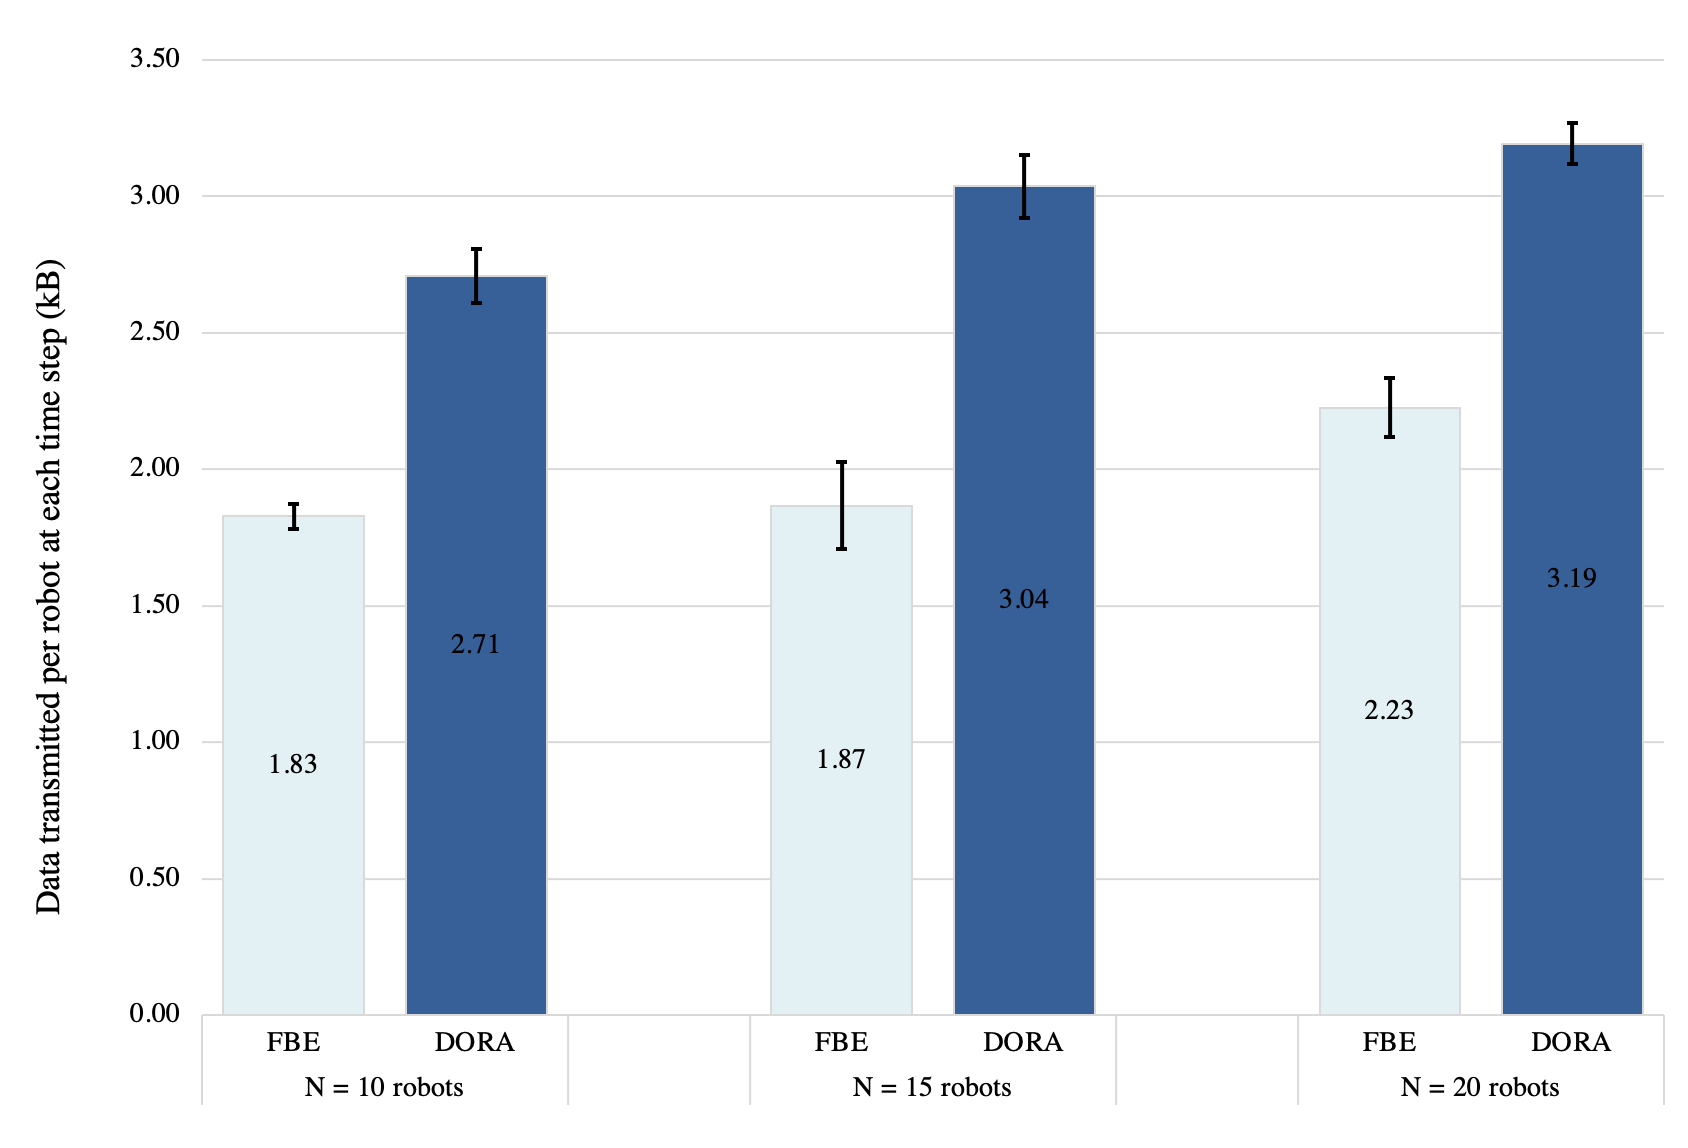
\includegraphics[width=0.97\columnwidth]{images/communication.png}
    \caption{Communication costs for DORA-Explorer and FBE}
    \label{results:communicationCosts}
\end{figure}

Results from Fig. \ref{results:parameters} show the performance of DORA-Explorer with varying ratios of risk gain $\alpha$ to exploration gain $\beta$. The experiments were carried with 10 robots. Results show that the number of remaining active robots at the end of the simulation only increases with a higher ratio. This is the expected behaviour as increasing the ratio corresponds to giving more importance to the risk avoidance gain from (\ref{eq:movement}). As for the number of cells explored, the relationship is not monotonic. In our experiments, a ratio $\alpha / \beta = 2$ provided the best result in terms of number of cells explored. For lower ratios, the robotic team is increasingly impacted by failures which in turns worsen the exploration performance. For higher ratios, the robot are too careful and don't explore as much the environment.

\begin{figure}[h]
    \centering
    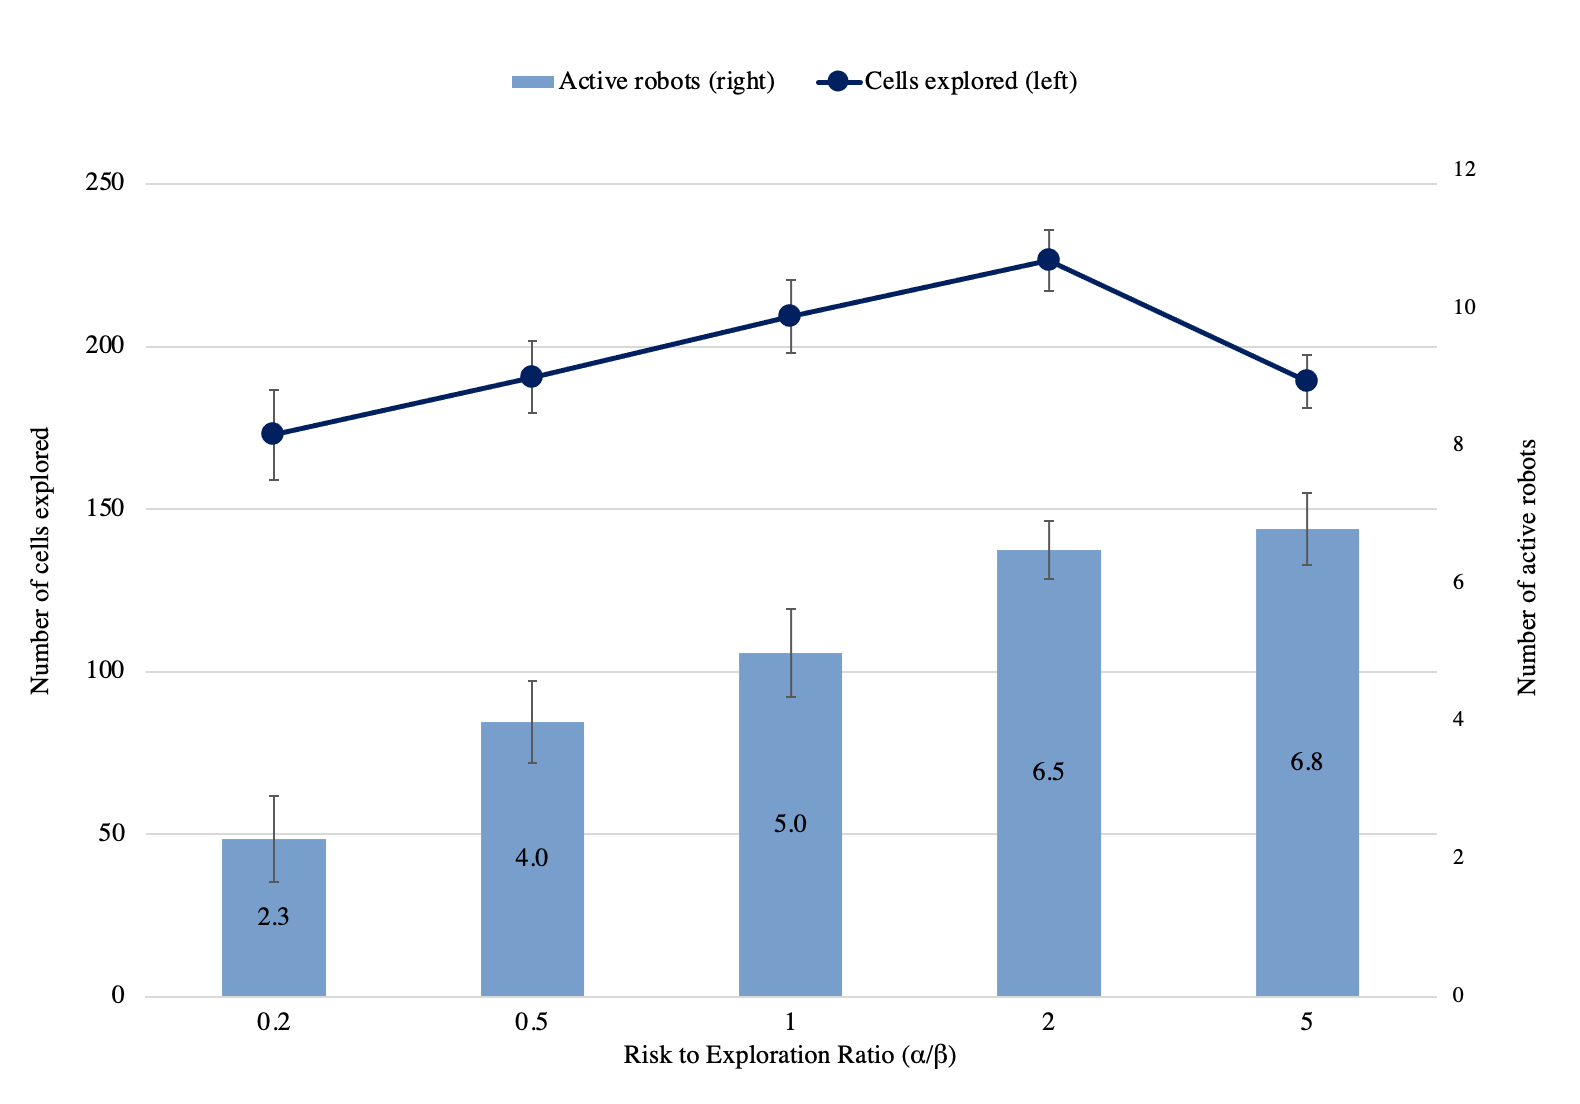
\includegraphics[width=1\columnwidth]{images/parameter.png}
    \caption{Performance of DORA-Explorer with varying ratios of $\alpha/\beta$}
    \label{results:parameters}
\end{figure}


\section{Physical experiments}
\subsection{Experimental setup}
In addition to the extensive simulations conducted in ARGoS, we tested
our system on a team of three physical KheperaIV robots in a 2x2m
environment containing 1 point radiation source. The environment is discretized as a 10x10 grid, meaning that each of
the 100 cells of the grid is 20x20cm large. Because the arena in
which we conducted the experiments was already limited in terms of
space we decided not to add obstacles.
Positioning of the
robots is done using an OptiTrack motion capture system. Radiation sensing is emulated
by an on board controller that reads the distance between the robot
and the radiation source to determine the current radiation
level. Failures are then triggered using equation \eqref{eq:failure}. If a robot fails, it stops moving and stops contributing to the exploration effort. The point
radiation source is located in a corner of the arena and the robots
are initially placed in the three remaining corners. We performed 5 runs over
200 steps of the DORA-Explorer algorithm. Each time step lasts 1s. Again, to assess DORA-Explorer's performance, we compare it to the results obtained by FBE and random
walk algorithms.

% \begin{figure}[h]
%     \centering
%     \captionsetup{belowskip=0pt}
%     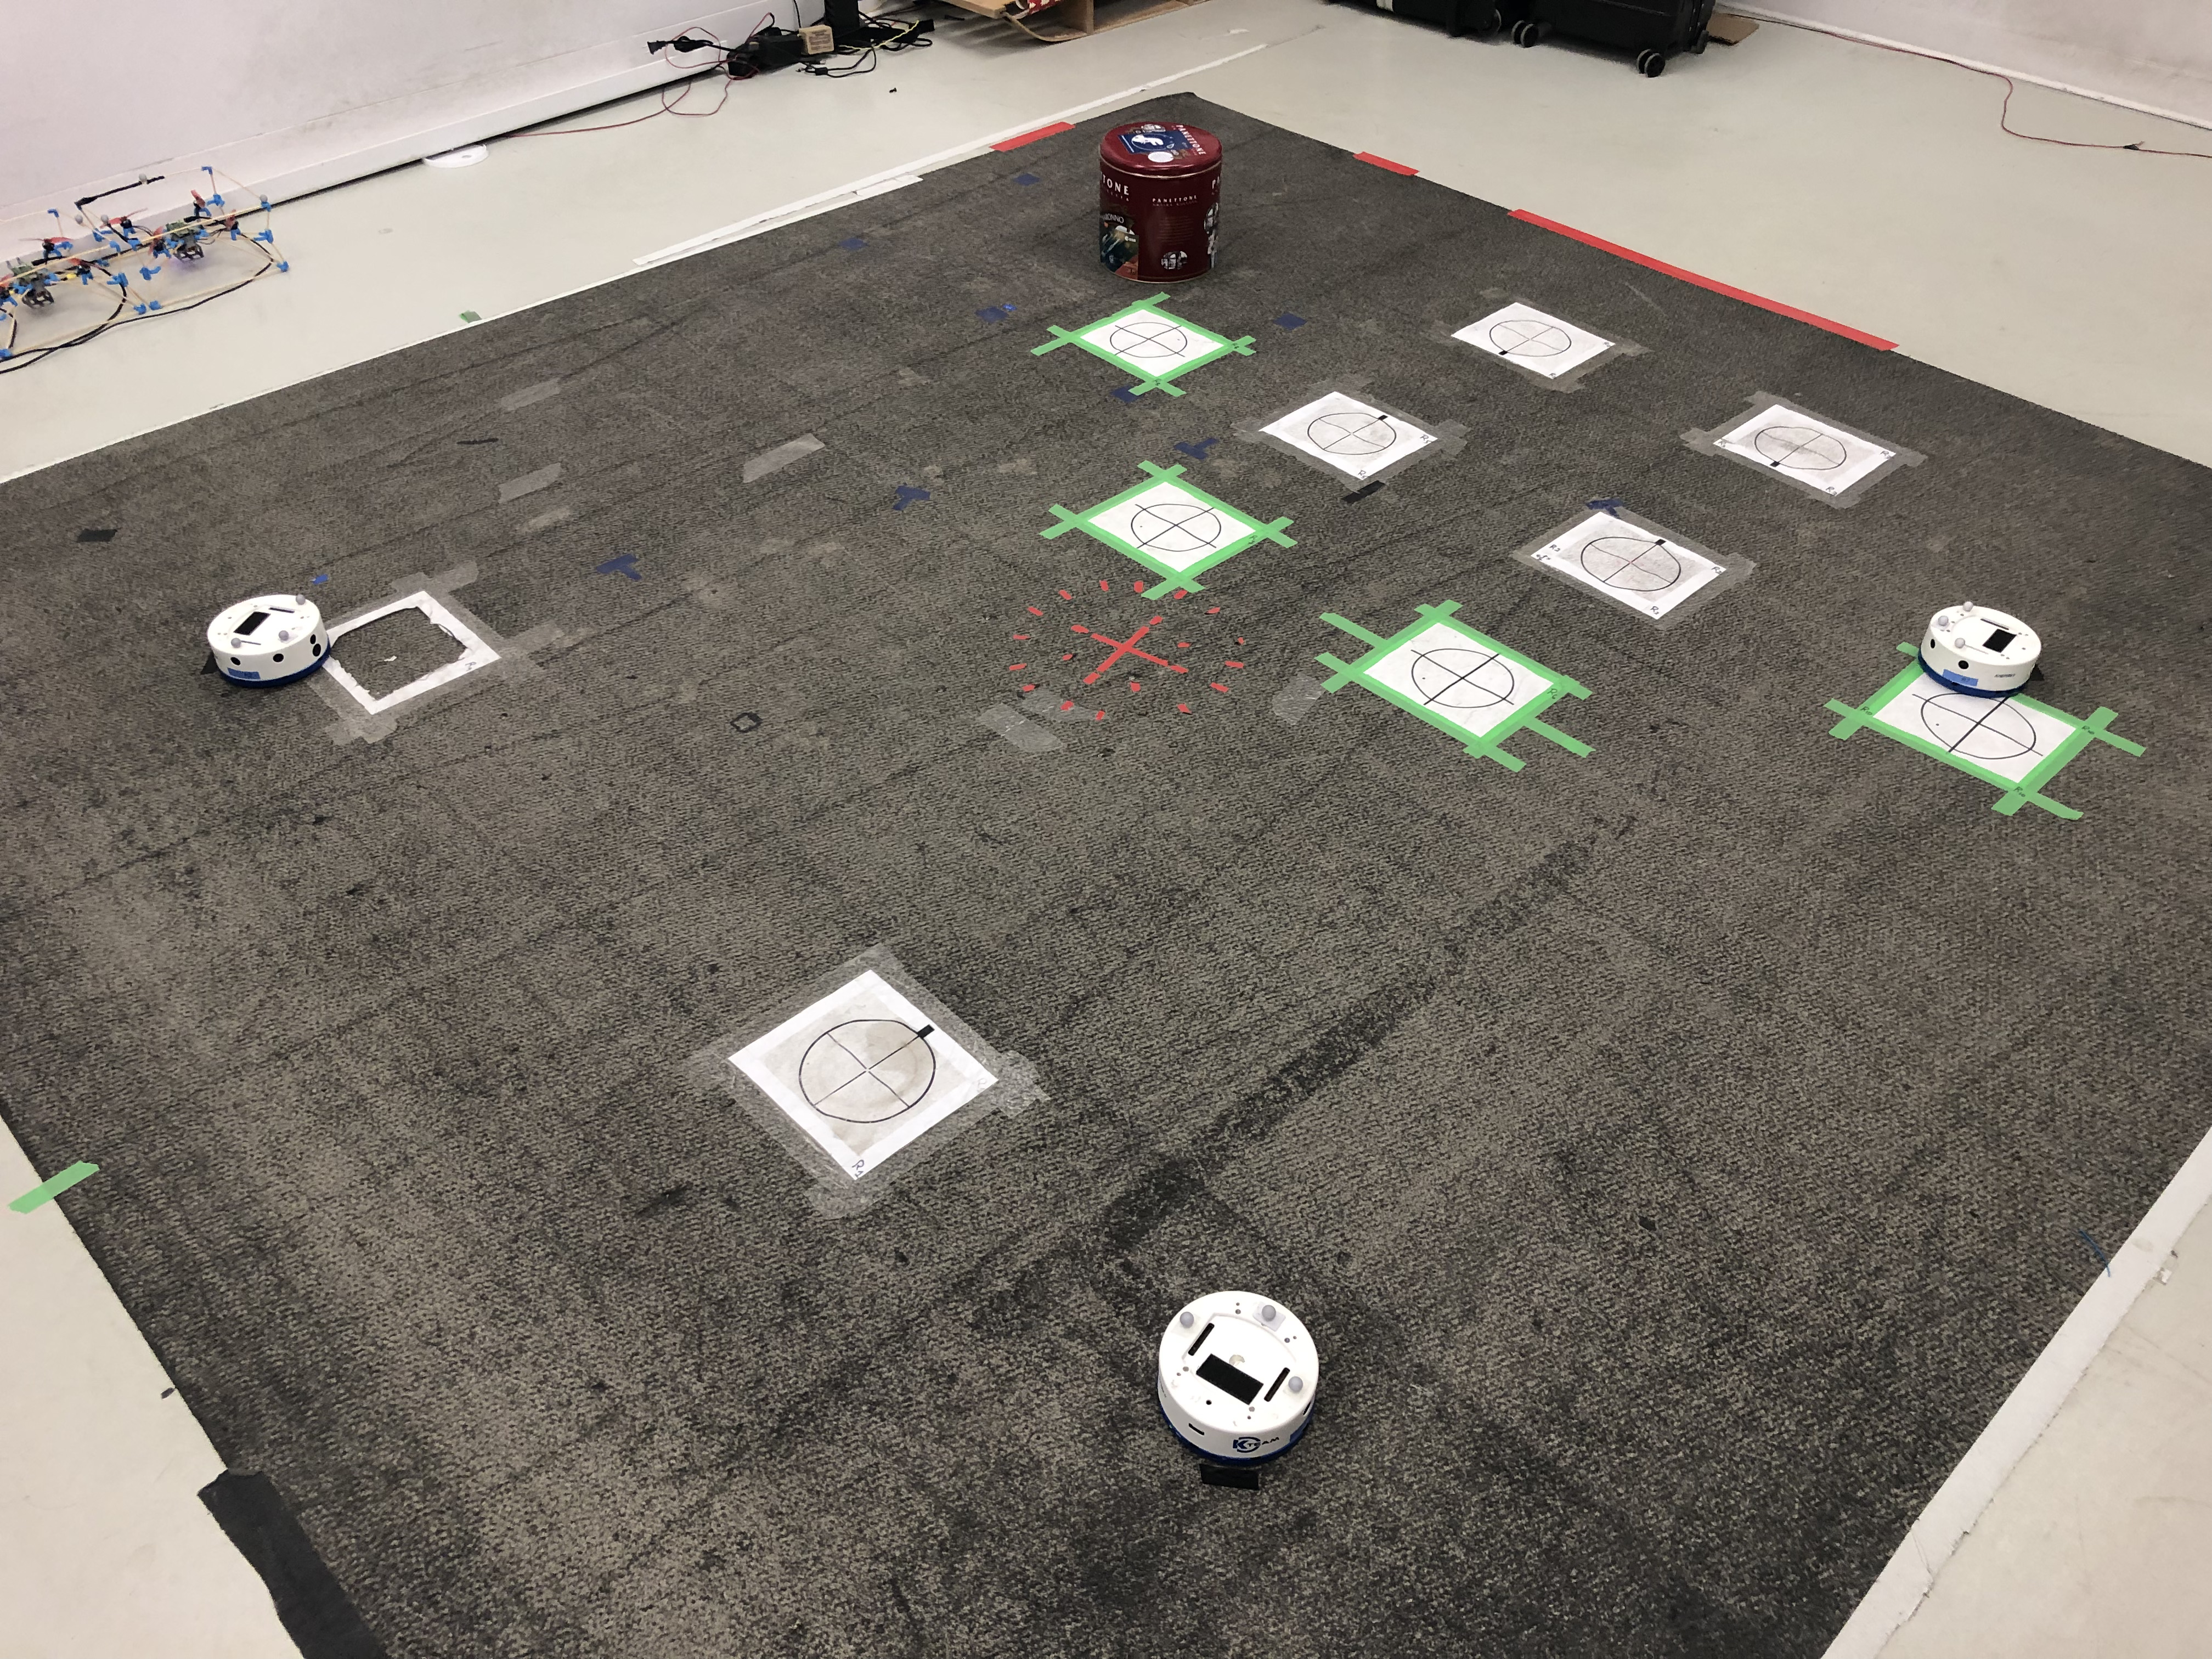
\includegraphics[width=0.65\columnwidth]{images/arena.jpeg}
%     \caption{Experiments on three physical KheperaIV robots. The red canister represents the point radiation source in the environment.}
%     \label{arena}
% \end{figure}


\subsection{Results}
The following results are an average of the 5 runs of each algorithm on physical robots.

\begin{figure}[H]
    \centering
    \captionsetup{belowskip=-5pt}
    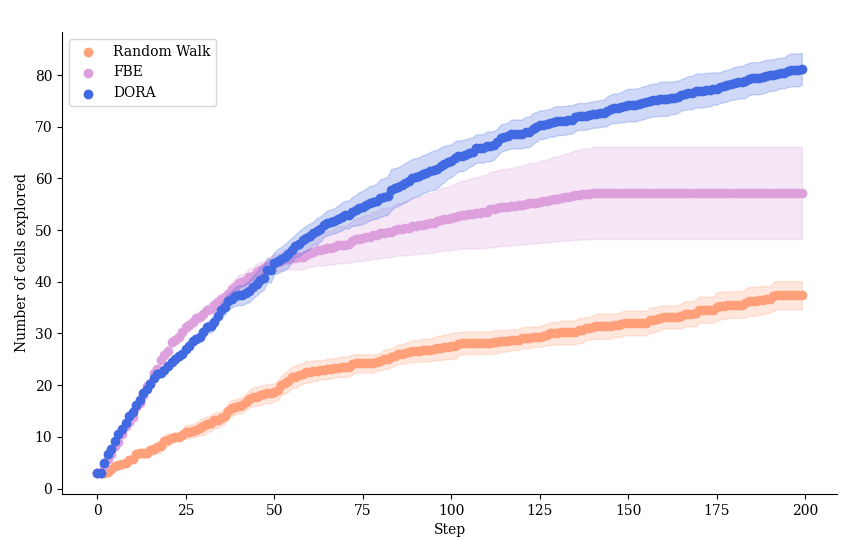
\includegraphics[width=0.82\columnwidth]{images/explored.png}
    \caption{Performance comparison of DORA-Explorer, FBE and random walk for number of explored cells over time on physical robots.}
    \label{results:cells_explored_physical}
\end{figure}

\begin{figure}[H]
    \centering
    \captionsetup{belowskip=-5pt}
    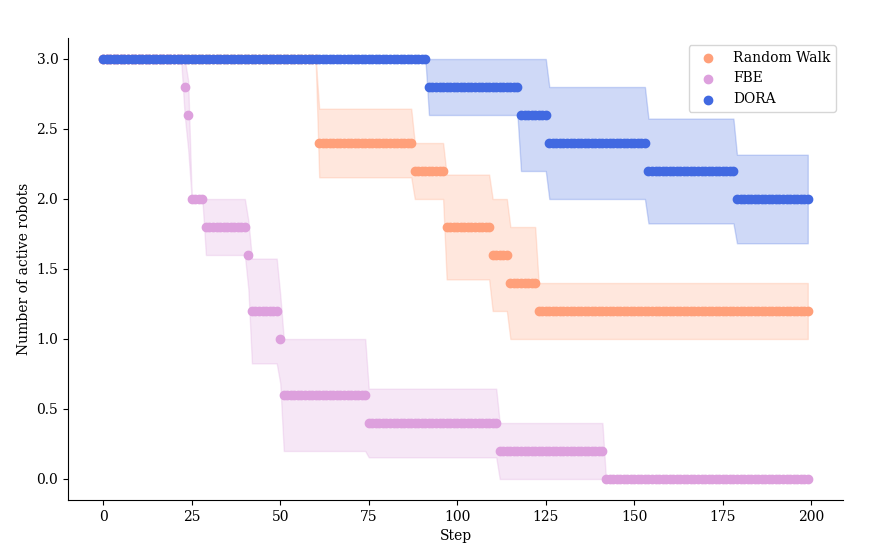
\includegraphics[width=0.82\columnwidth]{images/activerobots.png}
    \caption{Performance comparison of DORA-Explorer, FBE and random walk for number of active robots over time on physical robots.}
    \label{results:active_robots_physical}
\end{figure}

At the beginning of the exploration process, DORA-Explorer and FBE perform
similarly in terms of number of cells explored as shown in
Fig. \ref{results:cells_explored_physical}. The random walk
algorithm's exploration rate is considerably lower which can be
attributed to the fact that some of the cells of the environment are
visited multiple times: robots sometimes come back to positions that
they just had visited since their motion is determined randomly. As
time progresses, DORA-Explorer starts showing better exploration results than
FBE and at the end of the runs DORA-Explorer achieves a considerably better
coverage. Both FBE and DORA-Explorer clearly outperform the random walk
algorithm. In terms of robot failures, DORA-Explorer outperforms both FBE and the random
walk algorithm. This is shown in
Fig. \ref{results:active_robots_physical}, where DORA-Explorer exhibits a
higher level of active robots over time. When using FBE, all three
robots always fail before the end of the experiment. Random walk
shows a level of active robots that is in between DORA-Explorer and FBE. The results show that while DORA-Explorer and FBE initially have similar performances, as time progresses,
DORA-Explorer gets better when compared to FBE. The trend between DORA-Explorer and FBE in the physical experiments is inverted in comparison with the simulations because of the small environment into which the physical experiments were carried. Indeed, the likeliness of getting close of the radiation source was high, and as a result, without risk-awareness, the robots would fail very quickly. Because FBE
experiences a lot of failures, the failed robots stop exploring causing the exploration rate to decrease dramatically. In fact, FBE
always loses all its robots before the end of the experiments. In contrast,
DORA-Explorer keeps most of its robots active throughout the experiment and as a result the exploration rate remains high.


\section{Conclusion}
We presented DORA-Explorer, a novel lightweight risk-aware exploration
algorithm that minimizes the risk to which robots expose themselves in
order to maximize the amount of ground they will be able to cover. We expected that our exploration algorithm, which
leverages DBMs, would greatly outperform non-coordinated solutions,
and this has been the case. Indeed, it succeeded in reducing
considerably the likeliness of robot failures while keeping similar
ground coverage performance compared to other solutions proposed in
the literature. DORA-Explorer also showed good scalability thanks to its low
communication costs and its decentralized nature. It also showed applicability to real world
scenarios through experiments with physical robots. 

Taking inspiration from obstacle avoidance algorithms for the purpose of risk-avoidance could be an interesting future direction. Other future works include allowing DORA-Explorer to become more
or less risk-avoiding depending on the changing needs of the
situation. For example, in a search-and-rescue scenario, an increasing
urgency to rescue victims could motivate the willingness to take more
risks as time progresses. Also, more experiments could be conducted by
testing DORA-Explorer on a larger team of physical robots exploring
larger outdoor environments. Further applications of DORA-Explorer could
include using the generated risk belief map to determine robots'
fitness to store data in distributed storage systems like SwarmMesh
\cite{majcherczykSwarmmesh2020}, with robots assigned to tasks in
dangerous regions being discouraged from storing sensitive
information. Finally, in this work we considered that risk could be sensed by an on-board sensor. However,
in some scenarios, the risk cannot be directly perceived by any
sensors. In these cases, the belief map could instead be constructed using the
previous failures of the agents by assigning risk to areas only where
failures have been detected in the past.
